\documentclass[12pt]{book}

\usepackage{amsmath} % AMS Math Package
\usepackage{amsthm} % Theorem Formatting
\usepackage{amssymb}	% Math symbols such as \mathbb
\usepackage{amsmath} % AMS Math Package
\usepackage{amsthm} % Theorem Formatting
\usepackage{amssymb}	% Math symbols such as \mathbb
\usepackage{graphicx} % Allows for eps images
\usepackage{multicol} % Allows for multiple columns
\usepackage[dvips,letterpaper,margin=1in,bottom=1in]{geometry}
%\usepackage{minted}

\usepackage[dvipsnames]{xcolor}
\usepackage{etoolbox}

\usepackage{standalone}
\usepackage{tikz,ifthen}
\usetikzlibrary{arrows,shapes,trees,backgrounds}
\usepackage{subcaption}
\usepackage{bbold}
\usepackage{hyperref}
\usepackage[makeroom]{cancel}
\usepackage{pdfpages}

\numberwithin{equation}{section}
\usepackage{amsthm}

\usepackage{anyfontsize}

\usepackage{adjustbox}
\usepackage{graphbox}
\usepackage{wrapfig}

\usepackage[toc,page]{appendix}

\usepackage{enumitem}

\usepackage{pifont}


% ***********************************************************
% ******************* PHYSICS HEADER ************************
% ***********************************************************
% Version 2

% \DeclareMathOperator{\Sample}{Sample}
\let\vaccent=\v % rename builtin command \v{} to \vaccent{}
\renewcommand{\v}[1]{\ensuremath{\mathbf{#1}}} % for vectors
\newcommand{\gv}[1]{\ensuremath{\mbox{\boldmath$ #1 $}}}
% for vectors of Greek letters
\newcommand{\uv}[1]{\ensuremath{\mathbf{\hat{#1}}}} % for unit vector
\newcommand{\abs}[1]{\left| #1 \right|} % for absolute value
\newcommand{\avg}[1]{\left< #1 \right>} % for average
\let\underdot=\d % rename builtin command \d{} to \underdot{}
\renewcommand{\d}[2]{\frac{d #1}{d #2}} % for derivatives
%\newcommand{\dd}[2]{\frac{d^2 #1}{d #2^2}} % for double derivatives
\newcommand{\pd}[2]{\frac{\partial #1}{\partial #2}}
% for partial derivatives
\newcommand{\pdd}[2]{\frac{\partial^2 #1}{\partial #2^2}}
% for double partial derivatives
\newcommand{\pdc}[3]{\left( \frac{\partial #1}{\partial #2}
 \right)_{#3}} % for thermodynamic partial derivatives
\newcommand{\ket}[1]{\left| #1 \right>} % for Dirac bras
\newcommand{\bra}[1]{\left< #1 \right|} % for Dirac kets
\newcommand{\braket}[2]{\left< #1 \vphantom{#2} \right|
 \left. #2 \vphantom{#1} \right>} % for Dirac brackets
\newcommand{\matrixel}[3]{\left< #1 \vphantom{#2#3} \right|
 #2 \left| #3 \vphantom{#1#2} \right>} % for Dirac matrix elements
\newcommand{\grad}[1]{\gv{\nabla} #1} % for gradient
\let\divsymb=\div % rename builtin command \div to \divsymb
\renewcommand{\div}[1]{\gv{\nabla} \cdot #1} % for divergence
\newcommand{\curl}[1]{\gv{\nabla} \times #1} % for curl
\let\baraccent=\= % rename builtin command \= to \baraccent
\renewcommand{\=}[1]{\stackrel{#1}{=}} % for putting numbers above =
\newtheorem{prop}{Proposition}
\newtheorem{thm}{Theorem}[section]
\newtheorem{lem}[thm]{Lemma}
\theoremstyle{definition}
\newtheorem{dfn}{Definition}
\theoremstyle{remark}
\newtheorem*{rmk}{Remark}

% ***********************************************************
% ********************** END HEADER *************************
% ***********************************************************


% This allows us to add our colors
\usepackage{xcolor}

%just input either solarized light or dark to change between the colors
% Background Tones
\definecolor{base3}{HTML}{002b36} % for solarized dark
\definecolor{base2}{HTML}{073642}
\definecolor{base02}{HTML}{eee8d5} % for solarized light
\definecolor{base03}{RGB}{253,246,227}

% Content Tones
\definecolor{base1}{HTML}{586e75}
\definecolor{base0}{HTML}{657b83}
\definecolor{base00}{HTML}{839496}
\definecolor{base01}{HTML}{93a1a1}

% Accent Colors
\definecolor{cyan}{HTML}{2aa198}
\definecolor{violet}{HTML}{6c71c4}
\definecolor{yellow}{HTML}{b58900}
\definecolor{orange}{HTML}{cb4b16}
\definecolor{red}{RGB}{220,50,47}
\definecolor{magenta}{HTML}{d33682}
\definecolor{blue}{HTML}{268bd2}
\definecolor{cyan}{HTML}{2aa198}
\definecolor{green}{HTML}{859900}

%% Background Tones
\definecolor{base03}{HTML}{002b36} % for solarized dark
\definecolor{base02}{HTML}{073642}
\definecolor{base2}{HTML}{eee8d5} % for solarized light
\definecolor{base3}{RGB}{253,246,227}

% Content Tones
\definecolor{base01}{HTML}{586e75}
\definecolor{base00}{HTML}{657b83}
\definecolor{base0}{HTML}{839496}
\definecolor{base1}{HTML}{93a1a1}

% Accent Colors
\definecolor{cyan}{HTML}{2aa198}
\definecolor{violet}{HTML}{6c71c4}
\definecolor{yellow}{HTML}{b58900}
\definecolor{orange}{HTML}{cb4b16}
\definecolor{red}{RGB}{220,50,47}
\definecolor{magenta}{HTML}{d33682}
\definecolor{blue}{HTML}{268bd2}
\definecolor{green}{HTML}{859900}





\usepackage[many]{tcolorbox}
\tcbset
{every box/.style={colback=base03,colframe=blue,boxrule=2mm,bottom=-7pt},breakable}

% We will use this to alter commands and environments, making equations and tables different colors
\usepackage{etoolbox}
% All equation environments are base2
\AtBeginEnvironment{equation}{\color{base2}}
\AtBeginEnvironment{equation*}{\color{base2}}
\AtBeginEnvironment{math}{\color{violet}}
\AtBeginEnvironment{align}{\color{base2}}
\AtBeginEnvironment{tabular}{\color{violet}}
\usepackage{cancel}
\renewcommand{\CancelColor}{\color{red}}
\newcommand\Ccancel[2][\color{red}]{\renewcommand\CancelColor{\color{#1}}\cancel{#2}}

% A nice sans- serif font
\usepackage[default,osfigures,scale=1]{opensans}

% Un-italicized the equations and makes them easier to read. Check out
% http://www.biwako.shiga-u.ac.jp/sensei/kumazawa/tex/newtx.html
% for more options
\usepackage{amsmath}
\usepackage{cmbright}

% Doesn't seem to be working in Share LaTeX
% Gives you control over footer, header, etc. so we can have a highlighter page number
% We also have the section title up on top
\usepackage{fancyhdr}
\pagestyle{fancy}
\cfoot{\textcolor{violet}{\thepage} }
\cfoot{\textcolor{violet}{\thepage} }
\fancyhead[L]{\textcolor{violet}{\slshape \leftmark}}
\fancyhead[R]{}

% Allows us to style section headings
\usepackage{sectsty}
\sectionfont{\color{yellow}}
\subsectionfont{\color{orange}}
\subsubsectionfont{\color{green}}

%Control over figure captions.  I bolded them as well
\usepackage[font={color=cyan,bf}]{caption}

\newtheorem{example}{Example}
\newtheoremstyle{defin}{3pt}{3pt}{\color{base0}}{}{\color{blue}\bfseries}{:}{  }{}
\theoremstyle{defin}
\newtheorem{definition}{Definition}
\newtheoremstyle{remar}{}{}{\itshape}{}{\color{violet}\bfseries}{}{ }{}
\theoremstyle{remar}
\newtheorem*{remark}{Remark}


\title{\textcolor{red}{Math doesn't need to be hard}\\
\textcolor{green}{\large A physicist's guide with pictures and handwaving}}
\author{Christina Lee}

%\includeonly{./svd}

\begin{document}

%\usemintedstyle{solarizedlight}


\pagecolor{base03}
\color{base1}
\maketitle


\tableofcontents


%\section{Spin in Magnetic Field}
The non-relativistic Hamiltonian for a free particle in a magnetic field
\begin{equation}
  \mathcal{H}=-\frac{\hbar^2}{2m}\left(\grad-i\frac{q}{c\hbar}\mathbf{A} \right)^2
\end{equation}
contains a dependence on a gauge field $\omega$, since the gradient of the any $\omega$ can be added to the the vector potential $\mathbf{A}$ without changing the physical magnetic field
\begin{equation}
  \mathbf{B}=\grad \times \left(\mathbf{A}+\grad \omega \right)=\grad \times \mathbf{A}
\end{equation}

Suppose that $\Psi (\mathbf{r})$ is a solution to the $\mathbf{A}=0$ non-magnetic situation.  Then
\begin{equation}
  \Psi^A(\mathbf{r}) = e^{i\frac{q}{c\hbar} \int_{\mathbf{r}_0}^{\mathbf{r}} \mathbf{A}(\mathbf{r}^{\prime}) \cdot d\mathbf{r}^{\prime}   }
  \Psi(\mathbf{r})
\end{equation}
is a solution to the general vector potential $\mathbf{A}\neq 0$ Hamiltonian.
For ease, let $i\frac{q}{c\hbar} \int_{\mathbf{r}_0}^{\mathbf{r}} \mathbf{A}(\mathbf{r}^{\prime}) \cdot d\mathbf{r}^{\prime} = \phi$.
\begin{subequations}
  \begin{equation}
    \grad^2  -\left(\frac{q}{c\hbar}\right)^2\mathbf{A}^2
    -i\frac{q}{c\hbar} \mathbf{A} \grad
    -i \frac{q}{c \hbar} \left((\grad \mathbf{A}) + \mathbf{A}\grad \right)
   \end{equation}
   \begin{equation}
     \grad^2  -\left(\frac{q}{c\hbar}\right)^2\mathbf{A}^2
     -2 i\frac{q}{c\hbar} \mathbf{A} \grad
     -i \frac{q}{c \hbar} \left(\grad \mathbf{A}\right)
   \end{equation}

   Calculating a $\grad$
   \begin{equation}
     \left(i \frac{q}{c \hbar} \right) \mathbf{A}
     e^{\phi} \Psi (\mathbf{r}) +
     e^{\phi} \grad \Psi (\mathbf{r})
   \end{equation}
   Taking just the $\grad^2$ term
   \begin{equation}
     e^{\phi} \left(
    \grad^2 \Psi(\mathbf{r})
     +
    2\frac{i q}{c \hbar} \mathbf{A} \grad \Psi(\mathbf{r})
     -
     \left(\frac{q}{c\hbar}\right)^2 \mathbf{A}^2  \Psi(\mathbf{r})
     +
     \frac{i q}{c \hbar}
      \Psi(\mathbf{r}) \grad \mathbf{A} \right)
   \end{equation}
\end{subequations}


\chapter{Introduction}

Mathematics uses a precise language, and that's not a language we learn unless we specifically take classes catered to either mathematicians or philosophers.  The language emphasizes exact precision and logic.  The definitions, theorems, proofs: they all are meticulously crafted to leave no opening for ambiguity.  Everything needs to be precisely defined.  If you are unused to this language, check out Appendix~\ref{ch:notation} for some of the shorthand we use.

Humans don't naturally think this way.  Only by reading and writing a lot of technical math, feeling stupid for a long time, and turning your brain to a pile of mush can you train your mind to work at this higher level of precision.  That way of thinking will not just benefit your mathematics skills, but your all-around ability to precisely define concepts and problems in any situation.  Precision and logical progression can help most difficulties.

The other day, I was playing a grammar game, where I had to decide if a particular sentence was correct or not.  The sentence was, "He stole the blue woman's purse".  With my mathematical thinking, I got the question wrong, because technically, nothing is wrong with having a "blue woman".  Precisely, the sentence was grammatically correct.  Just much less probable than the person intending "He stole the woman's blue purse".  That's the difference between mathematical thinking and conventional thinking.

A joke runs about a biologist, a physicist, and a mathematician traveling through Ireland when they spot a flock of white sheep.  The biologist concludes that "Sheep in Ireland are white".  The physicist concludes that "Some sheep in Ireland are white".  The mathematician concludes that "At least one side of some sheep in Ireland are white".

But at the end of the day, all of this abstract language terms serve to convey a beautiful wonderland that just \textit{can't} be adequately described through any other wording.  It's like trying to describe blue to a blind person or a statue to someone who lives in two dimensions.  Each person needs to get to the idea for themselves through hard work.

Yet most sources assume that since precise definitions are ``necessary'', they are also ``sufficient''.  That means precise math talk is the only thing you get to go on. But I don't believe precise definitions are sufficient. So here, I will do my best to give you pictures, everyday examples, philosophical ponderings, jokes, and all the insights I've gained from my hours of intellectual masochism.

Enjoy.

\chapter{Sets and Maps}

A \textbf{Set} is one of the most basic structures we can construct in mathematics.

\begin{definition}[Set]
  A set is a collection of indistinguishable objects.
\end{definition}

The simplest set is the null set $ \emptyset = \{ \}$, the set that contains no objects.

Or we could have a set with one object, like $\{ \emptyset \}$, or $\{$\ding{36} $\}$.

We have two basic operations we can perform on sets, union and intersection.

\begin{definition}[Union]
  $c \in A \cup B$ if $a \in  A$ \textbf{OR} $a \in B$. $A\cup B$ is called the \textbf{union} of $A$ and $B$.
\end{definition}

\begin{definition}[Intersection]
  $c \in A \cap B$ if $a \in B$ \textbf{AND} $a \in B$.  $A \cap B$ is called the \textbf{intersection} of $A$ and $B$.
\end{definition}

Time for some examples:

Let $A = \{$\ding{40},\ding{88},\ding{101},\ding{161}$\}$ and $B= \{$ \ding{40}, \ding{39} $\}$.

Then $A \cup B = \{$\ding{40},\ding{88},\ding{101},\ding{161},\ding{39} $\}$.  And $A\cap B = \{$ \ding{40} $\}$.

You might notice I'm using weird shapes instead of numbers as members of my sets.  I don't want you to get stuck into thinking that these definitions and concepts only apply to abstract numbers and the sorts of things you dealt with in high school.  An investigator might very well look for the \textit{intersection} of those who where at Jimmy's bar on Friday night and The Pit on Saturday.  LGBTQ stands for the \textit{union} of Lesbians, Gays, Bisexuals, Transgenders, and Queers.

Seems fairly straightforward. But everything after that we do will be built on having a solid foundation in sets.

\begin{table}
\begin{tabular}{| c | c | c |}
  \hline
  Notation & Name & Example Elements \\
  \hline
  $\mathbb{R}$ & the Real line & 1, $\pi$, $\sqrt{2}$, $569543/3874329$, and $.3234898957786...$ \\
   $\mathbb{Z}$ & the Integers &  $-1, 0, 1, 2,...$ \\
  $\mathbb{Q}$ & The Rationals & $p/q : p,q \in \mathbb{Z}$ \\
  $S^1$ &  The surface of a circle. & $e^{i \phi} $ \\
  $S^2$ & The surface of a sphere. & \\
  \hline
\end{tabular}
  \caption{The names of some common special sets often encountered.}
  \label{tab:sets}
\end{table}



  Modern mathematics attempts to build up as much as possible just from sets.  Even our ideas of numbers

When we restrict our discussion of equivalence to just maps between sets, we get two important definitions,

\begin{definition}[Homomorphism]
  Given two sets $X$ and $Y$ with an algebraic structure on them $\circ$, for example multiplication, and a map between them $\phi:X\rightarrow Y$, $\phi$ is called a \textbf{homomorphism} and $X$ and $Y$ are said to be \textbf{homomorphic} to each other if $\phi$ preserves the structure on $Y$.  In other words, for $x_1,x_2 \in X$, $\phi(x_1)\circ \phi(x_2) = \phi(x_1 \circ x_2) \in Y$.
\end{definition}

Homomorphism just goes one way.  If we have this property in both directions, $X\rightarrow Y$ and $Y\rightarrow X$ we use the stricter condition of \textbf{Isomorphism},

\begin{definition}[Isomorphism]
  Given two sets $X$ and $Y$ with an algebraic structure on them $\circ$ and a map between them $\phi:X\rightarrow Y$, $\phi$ is called a \textbf{isomorphism} and $X$ and $Y$ are said to be \textbf{isomorphic} to each other if $\phi$ is homomorphic, and there exists an inverse $\phi^{-1}: Y \rightarrow X$ that is also homomorphic.
\end{definition}

\begin{figure}
  \begin{subfigure}{.25\textwidth}
    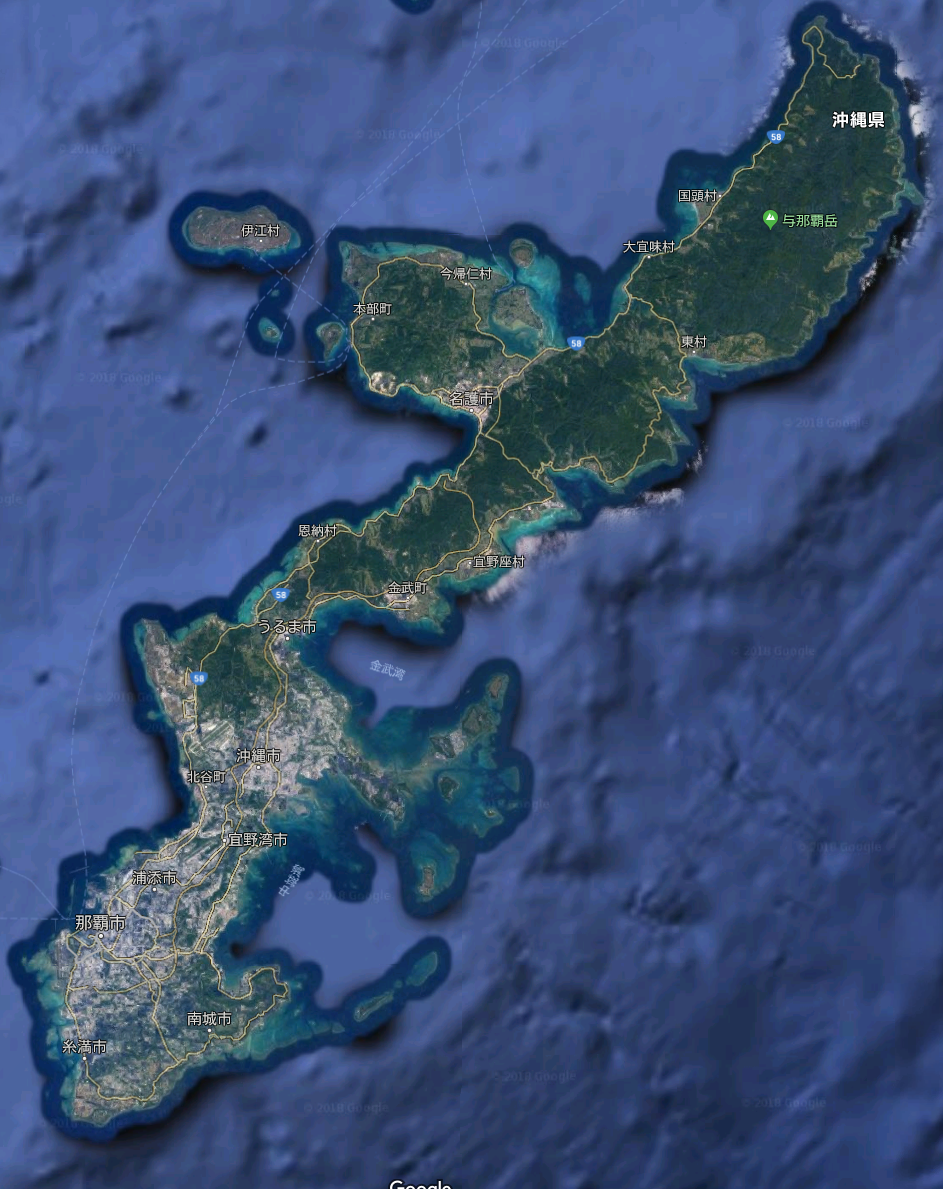
\includegraphics[width=\textwidth]{pics/okinawa.png}
    \caption{}
    \label{fig:okinawa}
  \end{subfigure}
  \begin{subfigure}{.25\textwidth}
    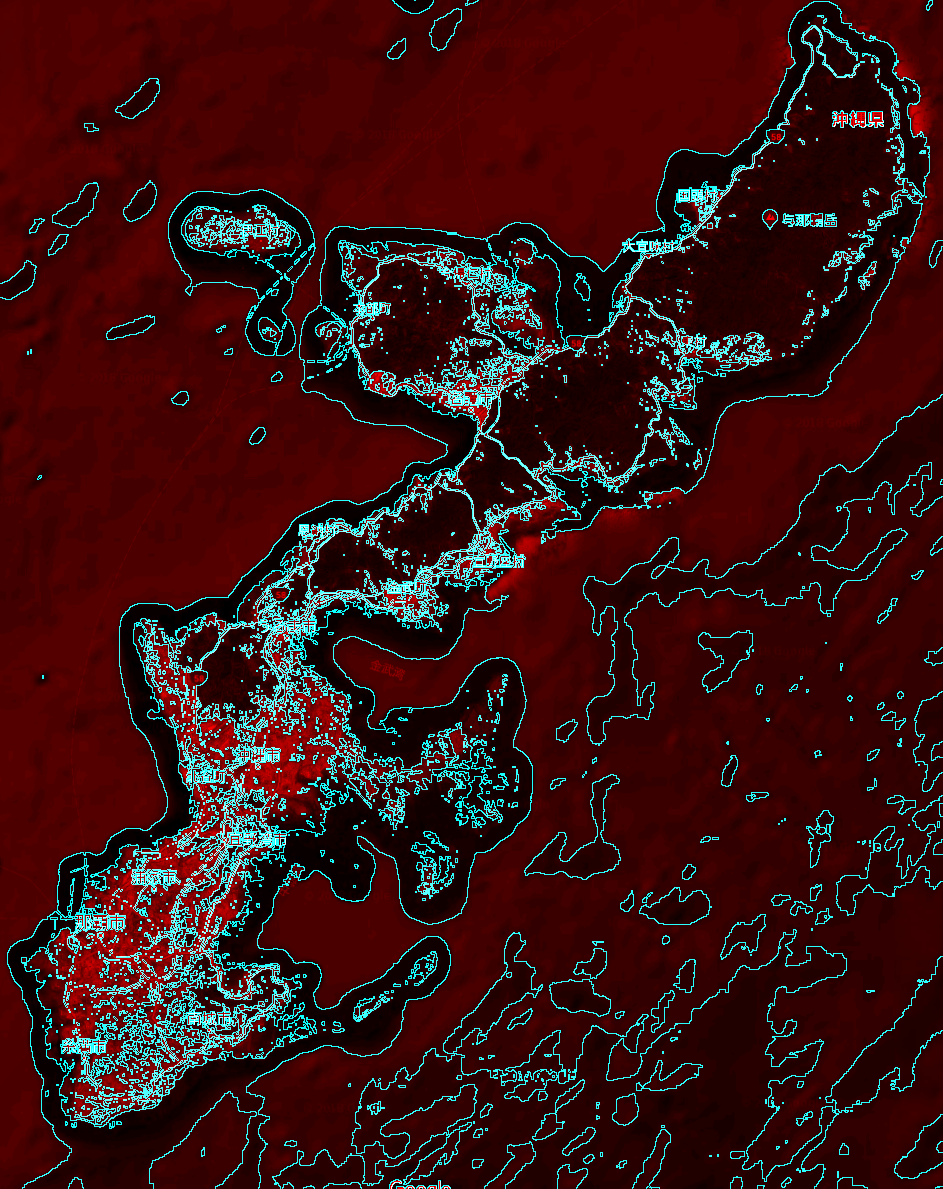
\includegraphics[width=\textwidth]{pics/okinawa_lines.png}
    \caption{}
    \label{fig:okinawa_lines}
  \end{subfigure}
  \begin{subfigure}{.25\textwidth}
    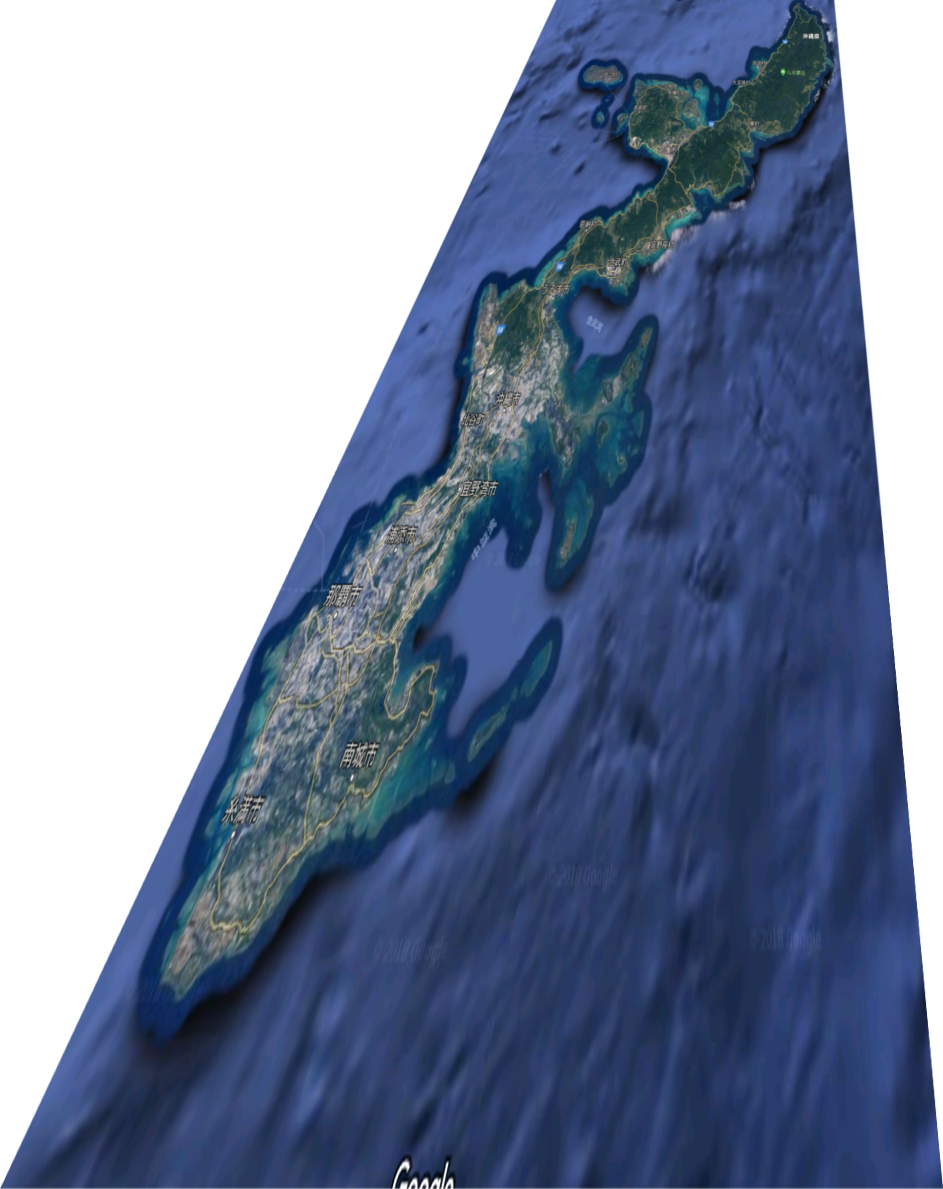
\includegraphics[width=\textwidth]{pics/okinawa_distort.png}
    \caption{}
    \label{fig:okinawa_distort}
  \end{subfigure}
  \caption{\ref{fig:okinawa} and \ref{fig:okinawa_lines} are only homomorphic to each other, since \ref{fig:okinawa} cannot be reconstructed from \ref{fig:okinawa_lines}.  \ref{fig:okinawa} and \ref{fig:okinawa_distort} are isomorphic in addition to being homomorphic since they are merely distortion of each other.  No information was lost.  }
\end{figure}

\chapter{Comparing Objects}\label{sec:comp}

\section{Equivalence Relations}

Mathematicians have some precise words to say whether something is identical to, indistinguishable from, or just for all intents and purposes equivalent to something else.  So let's go over those words.

\begin{definition}[Equivalence Relation]
  An \textbf{Equivalence Relation} $ \sim $ is a property between two objects that is
  \begin{enumerate}
    \item \textbf{Reflexive} $a \sim a$
    \item \textbf{Symmetric} $a \sim b \rightarrow b \sim a$
    \item \textbf{Transitive} If $a\sim b$ and $b \sim c$ then $a \sim c$
  \end{enumerate}
\end{definition}

Say my equivalence relation is ``is the same color as".  Then
\begin{itemize}
  \item ocean $ \sim $ sky
  \item grass $ \sim $ trees
  \item sunburn $ \sim $ lobster
\end{itemize}

Or I could use an equivalence relation that is "could be deformed into without cutting, tearing, or gluing".  Then

\begin{tabular}{c c c}
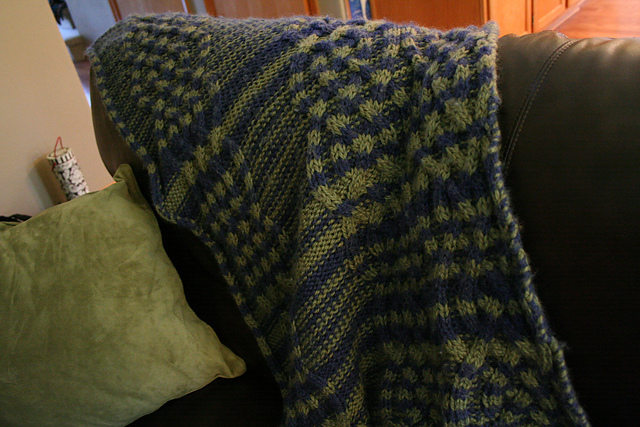
\includegraphics[width=.4\textwidth,align=c]{pics/shawl.JPG} & {\fontsize{50}{60}\selectfont $\sim$} & 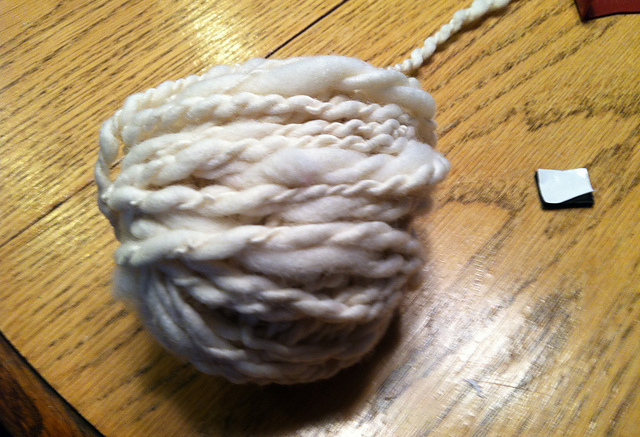
\includegraphics[width=.4\textwidth,align=c]{pics/yarn.JPG} \\
\end{tabular}

Let's treat these as ``ideal" objects, and forget about the fact the shawl is created from multiple different yarns, and that yarn itself is constructed from a vast number of individual fibers.


\begin{tabular}{c c c c c}
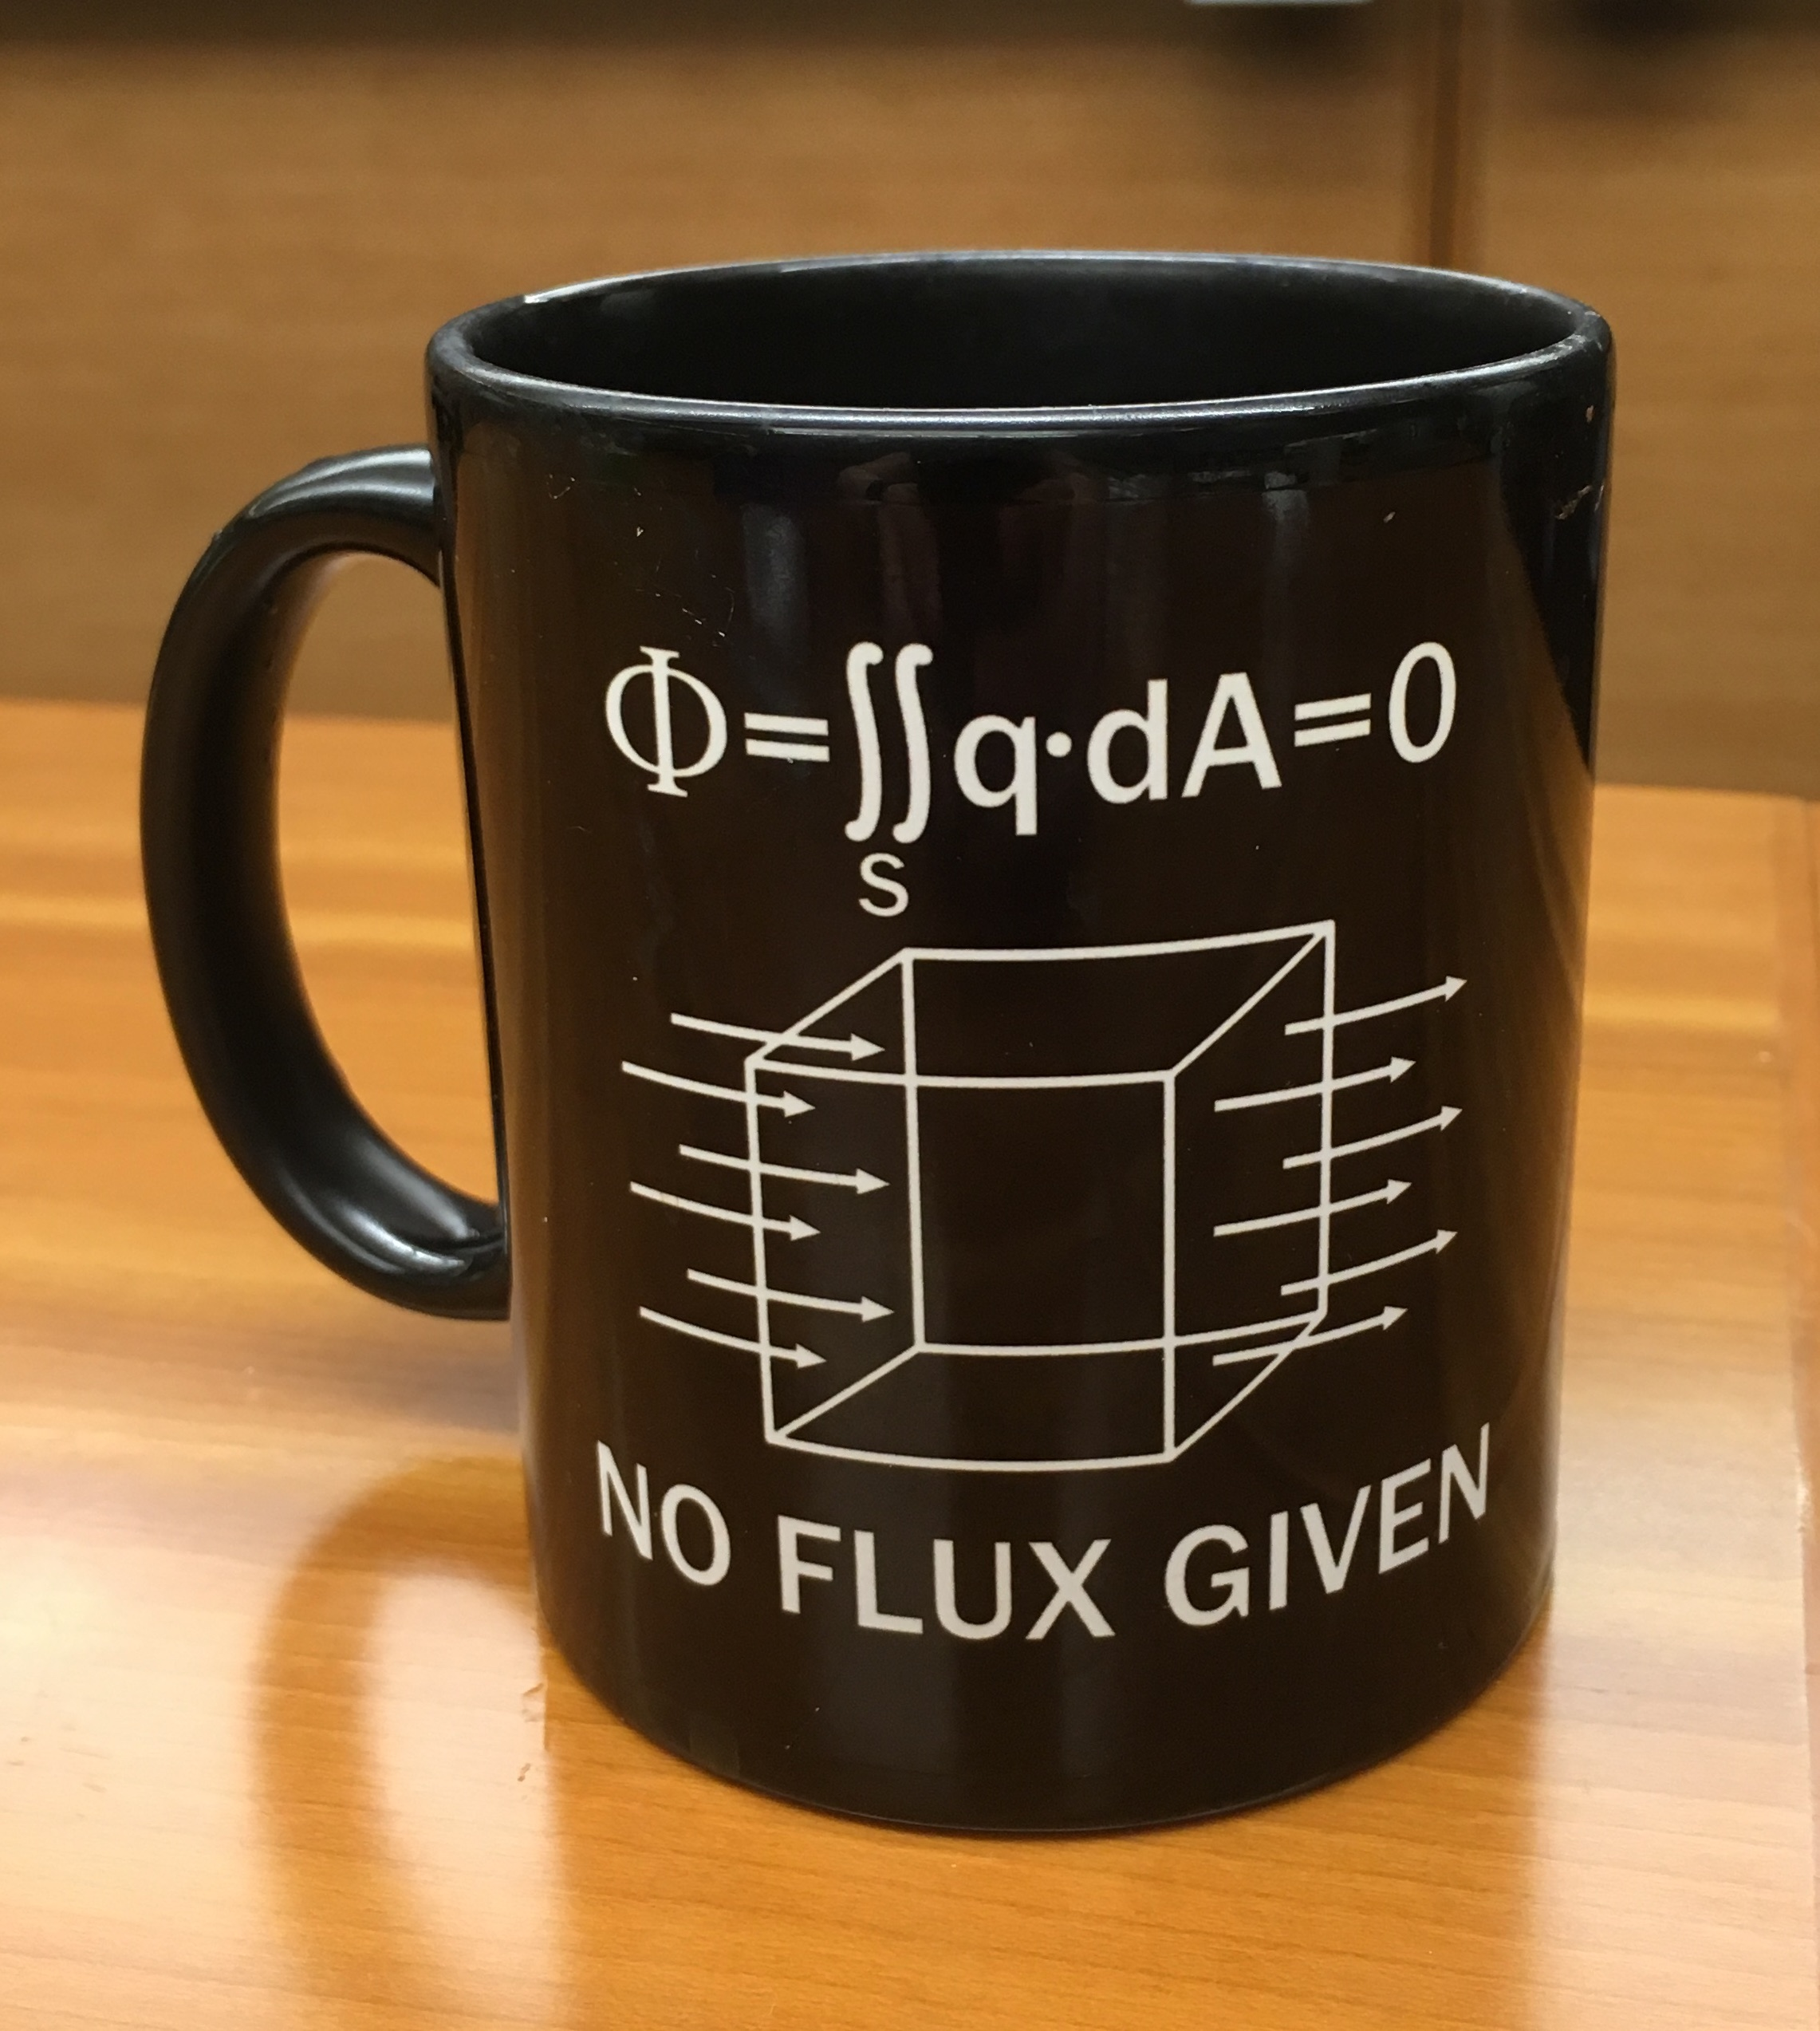
\includegraphics[width=.2\textwidth,align=c]{pics/mug.JPG} &
{\fontsize{50}{60}\selectfont $\sim$} &
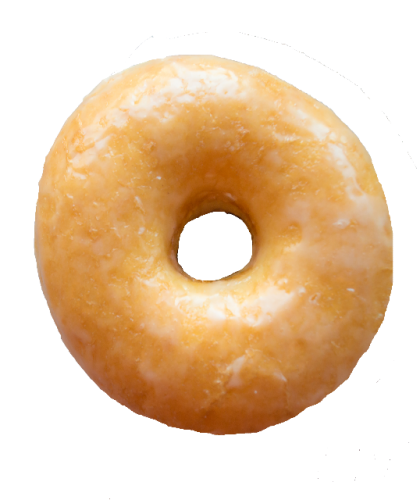
\includegraphics[width=.2\textwidth,align=c]{pics/donut.png}\protect\footnotemark &
{\fontsize{50}{60}\selectfont $\nsim$} &
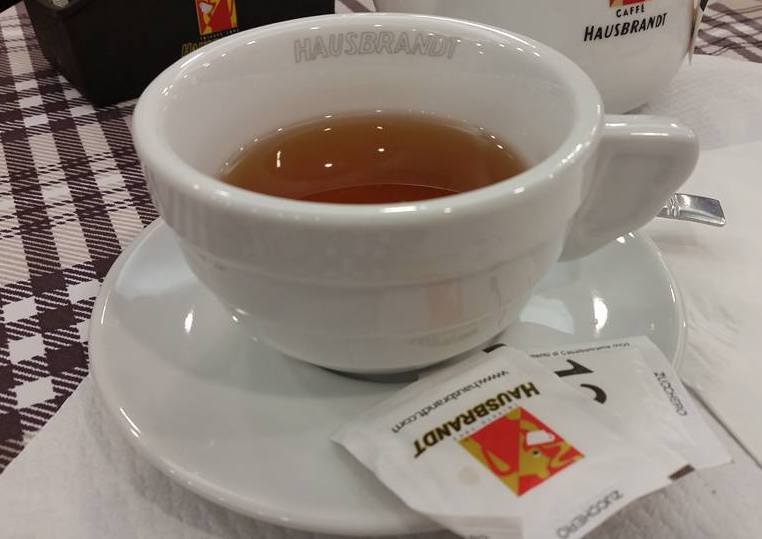
\includegraphics[width=.2\textwidth,align=c]{pics/not_a_donut.jpg} \\
\end{tabular}
\footnotetext{ http://pngimg.com/download/32474/?i=1}

\section{Equivalence Classes}

An equivalence relation can be used to define \textbf{equivalence classes}.

\begin{definition}[Equivalence Class]
  Given a set $S$ and a equivalence relation $\sim$ on elements in $S$, given an element $a\in S$, the \textbf{equivalence class} $[ a ] = \{ b \in S | b \sim a\}$.
\end{definition}

For $[a]$, $a$ is called the \textit{character} of that specific equivalence class, but we can use difference characters to represent the same equivalence class.  For example, if $a\sim b$, then $[a]$ and $[b]$ are the same thing.

An equivalence classes groups a bunch of things together based on similarity.  For example, we could use the equivalence relation "is same food group".  Then [apple] would represent all fruits.  I could equally write [orange] and mean the exact same thing.  But [croissant] would represent a different equivalence class, one that makes loaves of bread, tarts, scones, and muffins indistinguishable.

We do this all the time, even if we don't know it has the formal mathematical name of ``equivalence class''.  The term ``whales'' is just our way of grouping into a pile all humpbacks, blue whales, and right whales, given the equivalence relationship, "eats same way".  Well, maybe the relationship has a few more qualifiers.

Given a set and an equivalence relation, we can create a new set whose members are equivalence classes.  For example, let's say our initial set is everything on Earth, and the equivalence relation is ``is the same color as''.  We would end up with a set where one element was ``blue things'', another ``red things'', another ``green things''.  For the purposes of this explanation, let's simplify everything by saying objects will be either blue or green or some other nice pure color, not like those paint swatches you see at a hardware store with 150 shades of white.

For a math example, let the set be Integers $\mathbb{Z}$ and the equivalence relation be ``same parity''.  $1 \sim 3 \sim 5 \nsim 2$.  Now we have a new set with two elements, $[1]$ and $[2]$.

\section{Quotient Space}

\begin{definition}[Quotient Space]
  A \textbf{Quotient space} $S/\sim$ for a set $S$ and an equivalence relation $\sim$ is the set formed by equivalences classes in $S$ under $\sim$.
\end{definition}

Going back to the Integers $\mathbb{Z}$ and the equivalence relation ``same parity'', $\mathbb{Z}/ \sim  \approx \mathbb{Z}_2$.  I use $\approx$ as the answer isn't the group $\mathbb{Z}_2$, but just equivalent to $\mathbb{Z}_2$.  Instead, it's a group composed of the elements $[1]$ and $[2]$, where each element is an equivalence class.  This distinction might seem like a silly bit of finicky-ness here. When we are dealing with a set of loops, later on, I want you to remember that each member of the set is a geometric thing, or a collection of geometric things, though we map those objects onto numbers to be able to quantify and say things about them.




So far, these have been fun little real-world examples, but our equivalence relations can also divide materials up into similar phases, divide Hamiltonians up into groups with the same symmetries, or identify all wavefunctions equivalent up to a phase.

\chapter{Groups}

\section{What is a Group?}

\begin{definition}[Groups]
  A set $G$ and an operation $\cdot$ form a \textbf{group} if and only if
  \begin{itemize}[noitemsep]
    \item \textbf{Closure} $\forall a,b \in G$, $a\cdot b \in G$
    \item \textbf{Associativity} $\forall a,b,c, \in G$, $(a \cdot b) \cdot c = a \cdot (b \cdot c)$
    \item \textbf{Existence of Indentity} $\exists a \in G$ such that $\forall b \in G$, $a \cdot b = b$.  Such $a$ is called the identity, denoted $\mathbb{I}$.
    \item \textbf{Existence of Inverse} $\forall a \in G$, $\exists a^{-1}$ such that $a^{-1} \cdot a = \mathbb{I}$.
  \end{itemize}
\end{definition}

Any types of objects can form the set.  Commonly we speak of these sets in terms of abstract numbers, for example addition on the set of real numbers, but this definition works on any collection of objects.


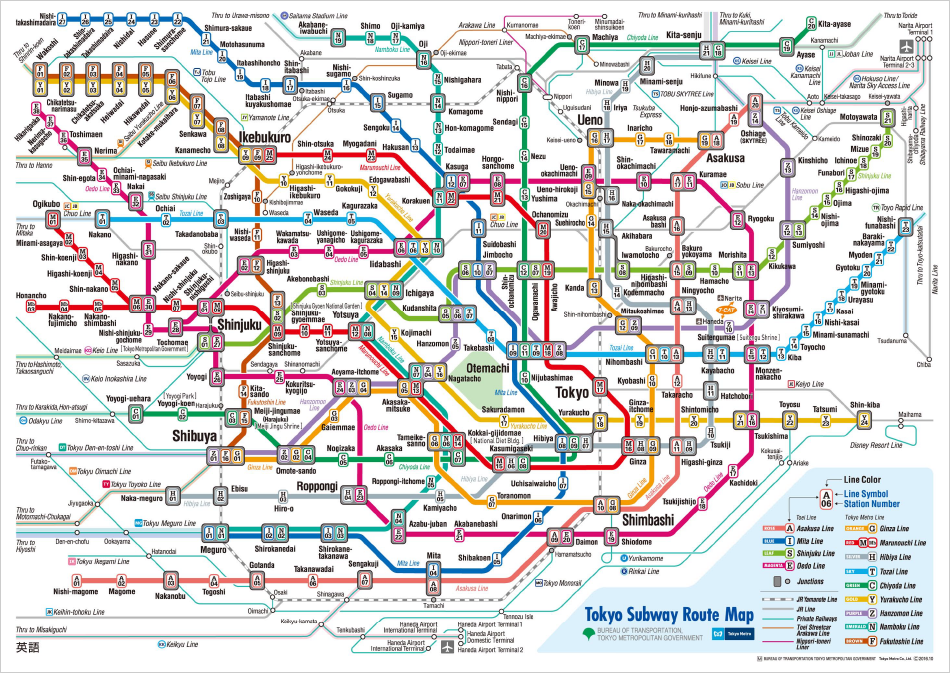
\includegraphics[width=\textwidth]{pics/tokyo_subway.png}
For example, take each path, even disjointed ones, you can take on the Tokyo subway as the element of a set. One element would be Shibuya $\rightarrow$ Shinjuku, another Shinjuku $\rightarrow$ Shibuya, yet another Asakusa $\rightarrow$ Akihabara.  Let's just assume specifying start and end points is enough to make the path deterministic, even though it totally isn't, especially for very confused tourists.  Once I have gone from one station to a new one, I can travel from the new station to a third.  Putting these two paths together is our composition operator $\cdot$.  For example, Ikebukuro$\rightarrow$ Shinjuku $\cdot$ Shinjuku $\rightarrow$ Shibuya .

If we only composed elements whose end points matched the start of the next, we would have a \textit{groupoid} rather than a group.   But we don't actually need the constraint that the end of one element has to match the start of the next.  For example, I could get into Tokyo at Shinjuku, then travel to Shibuya.  After wandering around and spending my year's worth of clothing budget, I might hop back on the subway at Harajuku to travel to Akihabara for some night life.  That element would be Shinjuku$\rightarrow$Shibuya$\cdot$ Harajuku$\rightarrow$Akihabara.  While Shibuya and Harajuku are fairly close together, what if I ran the Tokyo marathon? Or took an express bus to the airport, only to find out my plane was canceled and take the train back into the city?  I can compose paths arbitrarily far apart.

Let's work through requirements in the definition of a group.  Does this group obey \textbf{closure}?  Well, by combining any two routes in the metro, we still can't get anywhere the metro doesn't travel, so the composition will still be in the group.

How about \textbf{Associativity}?  The parentheses don't change how we will traverse the route, since we still tranverse the route left to right.  The parentheses only change how we \textit{plan} our route.  No matter how we plan, the start and end points will still end up being the same, and we will still have the same group object.

\textbf{Indentity}? One time in Akihabara, I couldn't figure out how to get to the locker where I stashed my luggage, so I had to pay to walk in one entrance and out a different exit.  In essence, I used the metro, but I didn't go anywhere.  I just applied the identity operation.  That exists for any station.

\textbf{Existance of Inverse}?  At least in this particular Metro, trains run both ways. This is a particularily nice feature for confused tourists who just jumped on a train before checking if it was the correct one. If I can travel A$\rightarrow$B, then I can travel B$\rightarrow$A.  If I combine those two paths, I get A$\rightarrow$B$\rightarrow$A = A$\rightarrow$A = I.

\section{Subgroups}

* Proper Subgroups

* Normal Subgroups

\section{Cosets of Subgroups}


\section{Quotient Groups}

* Conjugacy class

\chapter{Topology}

Topology is a minimal amount of structure put onto sets.  Once we have sets, we can start arranging the objects in them and assigning more information to the objects in the sets.

\begin{definition}[Topological Space] \label{def:topspace}
  A \textbf{Topological Space} is a set $X$ and a collection of subsets of $X$, $T$, such that
  \begin{enumerate}
    \item The empty set $\varnothing \in T$.
    \item $X \in T$.
    \item The intersection of a \textit{finite} number of sets in $T$ is also in $T$.
      \begin{equation}
        \cap_{T_i\in T}^{N < \infty} T_i \in T
      \end{equation}
    \item The union of \textit{up to an infinite number} of sets in $T$ is also in $T$.
      \begin{equation}
        \cup_{T_i \in T} T_i \in T
      \end{equation}
  \end{enumerate}
\end{definition}

\begin{example}[Trivial Topology]\label{ex:trivialtop} A \textbf{Trivial Topology} is when, for a given set $X$, the topology only contains $X$ and the null set $\varnothing$.

\begin{center}
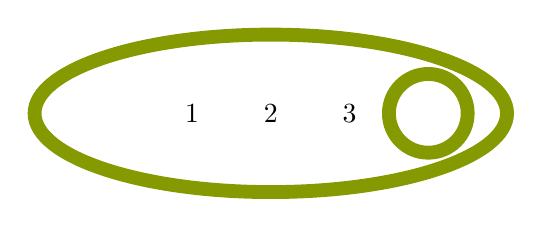
\begin{tikzpicture}
    \draw (-1,0) node{1};
    \draw (0,0) node{2};
    \draw (1,0) node{3};
    \draw[green, line width=5] (0,0) circle [ x radius = 3, y radius = 1];
    \draw[green, line width=5] (2,0) circle [x radius =.5, y radius = .5];
\end{tikzpicture}\end{center}
\end{example}

\begin{example}[Discrete Topology]\label{ex:discretetop} For a given set $X$, its \textbf{discrete topology} is the collection of all subsets of $X$.

\begin{center}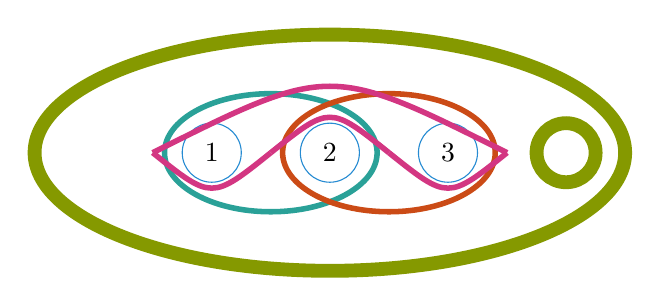
\begin{tikzpicture}[scale=1.5]
    \draw (-1,0) node{1};
    \draw (0,0) node{2};
    \draw (1,0) node{3};
    \draw[green, line width=5] (0,0) circle [ x radius = 2.5, y radius = 1];

    \draw[blue] (-1,0) circle [x radius =.25, y radius = .25];
    \draw[blue] (0,0) circle [x radius =.25, y radius = .25];
    \draw[blue] (1,0) circle [x radius =.25, y radius = .25];

    \draw[cyan, line width=2pt] (-.5,0) circle [x radius =.9, y radius = .5];
    \draw[orange, line width=2pt] (0.5,0) circle [x radius =.9, y radius = .5];

    \draw[magenta, line width=2pt] (-1.5,0) .. controls (0,.75) .. (1.5,0);
    \draw[magenta, line width=2pt] (-1.5,0) .. controls (-1, -.4) .. (-.5,0);
    \draw[magenta, line width=2pt] (-.5,0) .. controls (0,.4) .. (.5,0);
    \draw[magenta, line width=2pt] (.5,0) .. controls (1,-.4) .. (1.5,0);

    \draw[green, line width=5] (2,0) circle [x radius =.25, y radius = .25];
\end{tikzpicture}\end{center}
\end{example}

\begin{example}\label{ex:neithertop} Here's an example of a 3-element set that is neither the trivial nor discrete topology.

\begin{center}  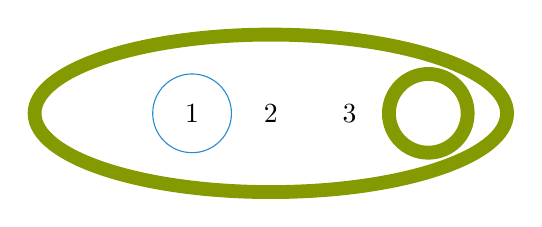
\begin{tikzpicture}
      \draw (-1,0) node{1};
      \draw (0,0) node{2};
      \draw (1,0) node{3};
      \draw[green, line width=5] (0,0) circle [ x radius = 3, y radius = 1];
      \draw[green, line width=5] (2,0) circle [x radius =.5, y radius = .5];

      \draw[blue] (-1,0) circle [x radius =.5, y radius = .5];
  \end{tikzpicture}\end{center}
\end{example}

We can also have topological spaces for continuous sets, like $\mathbb{R}$ or $\mathcal{S}^1$.

\begin{definition}[Open Ball]
  For $\epsilon > 0$, an \textbf{open ball} at point $p_1$ of radius $\epsilon$ is all points $B_{\epsilon}(p_1)= \{p_i | \abs{p_i - p_1}<\epsilon \}$.
\end{definition}

\begin{definition}[Standard Topology] \label{def:standardtop}
  The \textbf{Standard Topology} for a given set $X$ is the set, the null set, all open balls, and all finite unions of open balls.
\end{definition}

The standard topology is quite useful for limits and Calculus, since for any $\epsilon >0$, we can always find points $p_1, p_2$ such that $\abs{p_1 - p_2} <\epsilon$.

\section{Comparing Topologies}
In Section~\ref{sec:comp}, we defined two terms for comparing sets with an algebraic structure, \textit{homomorphism} and \textit{isomorphism}.  After we have attached a topology to the set, we have two analogous concepts with very confusing terminology.788

\begin{definition}[Homotopic]
  Two topologies are \textbf{homotopic} to each other if one can be continuously deformed into another, allowing for the collapse of dimensions and information loss.

  Officially, if there exists a function $F:X\times[0,1] \rightarrow Y$ that is continuous, then $X$ and $Y$ are homotopic.
\end{definition}

\begin{definition}[Homeomorphism]
  Two topologies $X$ and $Y$ are \textbf{homeomorphic} if there exists a function $f: X \rightarrow Y$ and inverse function $f^{-1}: Y \rightarrow X$ that are both continuous.
\end{definition}

The difference between \textit{homomorphic, homoemoprhic,} and \textit{homotopic} is tricky.  \textit{Homomorphic} and \textit{Isomorphic} are general categorization terms that apply to sets, research \textbf{Category Theory} for more information.  \textit{Hom\textbf{E}omorphic} applies specifically to topolog\textbf{Y} and geometr\textbf{Y}.

\section{Properties of Topologies}

While to prove two topologies homeomorphic, we need to find a map $f$ between them and it's inverse, we have more painless ways to prove that two topologies are not homeomorphic.  We have properties of topologies that are held invariant under isomorphism.  If we can show that two different topologies have different properties, then we know that they can't be isomorphic to each other.  If two topologies agree on every known property, then they probably are isomorphic to each other, but mathematicians love their counterexamples, so don't count on it.



\begin{definition}[Compact]
  A topology is called \textbf{compact} if every open cover has a finite subcover.
\end{definition}
That was the formal definition, but what does it mean?  Sometimes my desk seems like it has an infinite amount of papers spread out over it.  Let us suppose that my desk literally does have an infinite number of papers covering it.  I could take either a finite number of papers or an infinite number of papers to cover my desk, but either way, I could always find a finite subset of those that still cover the desk.

As opposed to my desk, the real line with the standard topology is not compact.  Suppose I choose the infinite cover of the real line $\mathbb{R}$,

\begin{center}

\begin{tikzpicture}[scale=2]
  \draw[green,->, line width=5] (-.25,.25) --  (-.75,.25);
  \draw[green,->, line width=5] (6.25,.25) -- (6.75,.25);
  \draw[magenta] (0,0) -- (6,0);
  \foreach \x in {0, 2, 4}
  { \draw[cyan, dashed] (\x,.25) -- (\x + 1.5,.25);
    \draw[cyan, dashed] (\x +1,.5) -- (\x +2.5,.5);}
\end{tikzpicture}
\end{center}

I have covered the real line with an infinite number of sets, but if I take even one away, $\mathbb{R}$ will no longer be covered.  The cover presented above does not have a \textit{finite} subcover.  Since \textit{every} cover has to have a finite subcover for a topology to be compact, we just to show one counter-example to show that a topology is not compact.  Hence, Reals equipped with the standard topology is not compact. QED.

Quod Erat Demonstrandum. Not Quantum Electro-Dynamics.  Much as I like me some relativistic light-matter interactions.

Moral of the story: don't play strip poker with the Real Numbers. If they started covered up, no matter how much they lose, there would always be more clothing to remove.

\begin{definition}[Hausdorff]
    Also known as \textbf{$T_2$}, every two points in a \textbf{Hausdorff} space have disjoint neighborhoods.
\end{definition}

\begin{definition}[Orientable]
  A topological space of dimension $n$ is said to be \textbf{Orientable} is it can be covered by a nowhere vanishing $n$-form.
\end{definition}
This $n$-form could potentially be the orientation of the space, though others might exist.



\subsection{Euler Character and Gauss-Bonnett Formula}

\section{Coordinate Systems}
Once we have a topology for a set, we can put even more information on the object via a coordinate system. At least in some circumstances. A topology gave us an idea of which objects are ``neighbors" and ``next to each other".  If two objects are usually in subsets together, then they are adjacent.  A coordinate system gives a precise way to quantify this.

So in what circumstances can we do this? When we are dealing with a \textbf{manifold}.

\begin{definition}[locally]
   If a condition holds \textbf{locally}, then for every point $p\in X$, $p$ is in some open set such that the condition holds on that open set.
\end{definition}

\begin{definition}[Manifold]
A \textbf{Manifold} is a topological space that locally looks like Euclidean space, $\mathbb{R}^n$, for some $n$.
\end{definition}

 The Standard Topology, ex.~\ref{def:standardtop}, could be a manifold, depending on the underlying set. For example, $X=\mathbb{R}$ equipped with the standard topology is a manifold, but the standard topology on a set like

\begin{center}
  
\begin{tikzpicture}
    \draw[line width=2, green] (-1,0) circle [x radius =1, y radius = .5];
    \draw[line width=2, green] (1, 0) circle [x radius =1, y radius = .5];
  \end{tikzpicture}
\end{center}

  is not a manifold because the point where the circles are joined no longer looks like a line.  Our other previous examples, ex.~\ref{ex:trivialtop},~\ref{ex:discretetop}, and \ref{ex:neithertop} are not manifolds as they are discrete.

\begin{definition}[Coordinate Chart]
  A \textbf{Chart} of a topology is a map $\phi: U \rightarrow V$, where $U$ is an open set in the topology, and $V$ is an open set in $\mathbb{R}^n$.   $\phi$ must be one-to-one and onto, thus defining a homeomorphism.
\end{definition}

\begin{definition}[Atlas]
  An \textbf{Atlas} is a collection of charts covering the entirity of a topological space.  If two charts overlap on a set $U \cap V$, where $\phi:U\rightarrow \mathbb{R}^n$ and $\psi:V\rightarrow \mathbb{R}^n$, then the transition function $\phi \circ \psi^{-1}: \mathbb{R}^n \rightarrow \mathbb{R}^n$ must be defined on $U\cap V$, be continuous, and be differentiable.
\end{definition}

See Fig~\ref{fig:atlas} for a conceptual idea of what an atlas and charts are.  While the mathematical terminology might seem strange and at odds with our conception from the English terms, the mathematical abstraction and everyday object have much in common.  The atlas is the comprehensive book of everything put together, all the charts.  We need more than one chart because I don't want United States highways at the same time I'm planning how to get around on the Tokyo subway.  Also, because latitude and longitude are ill-defined on the north pole.


\begin{figure}
  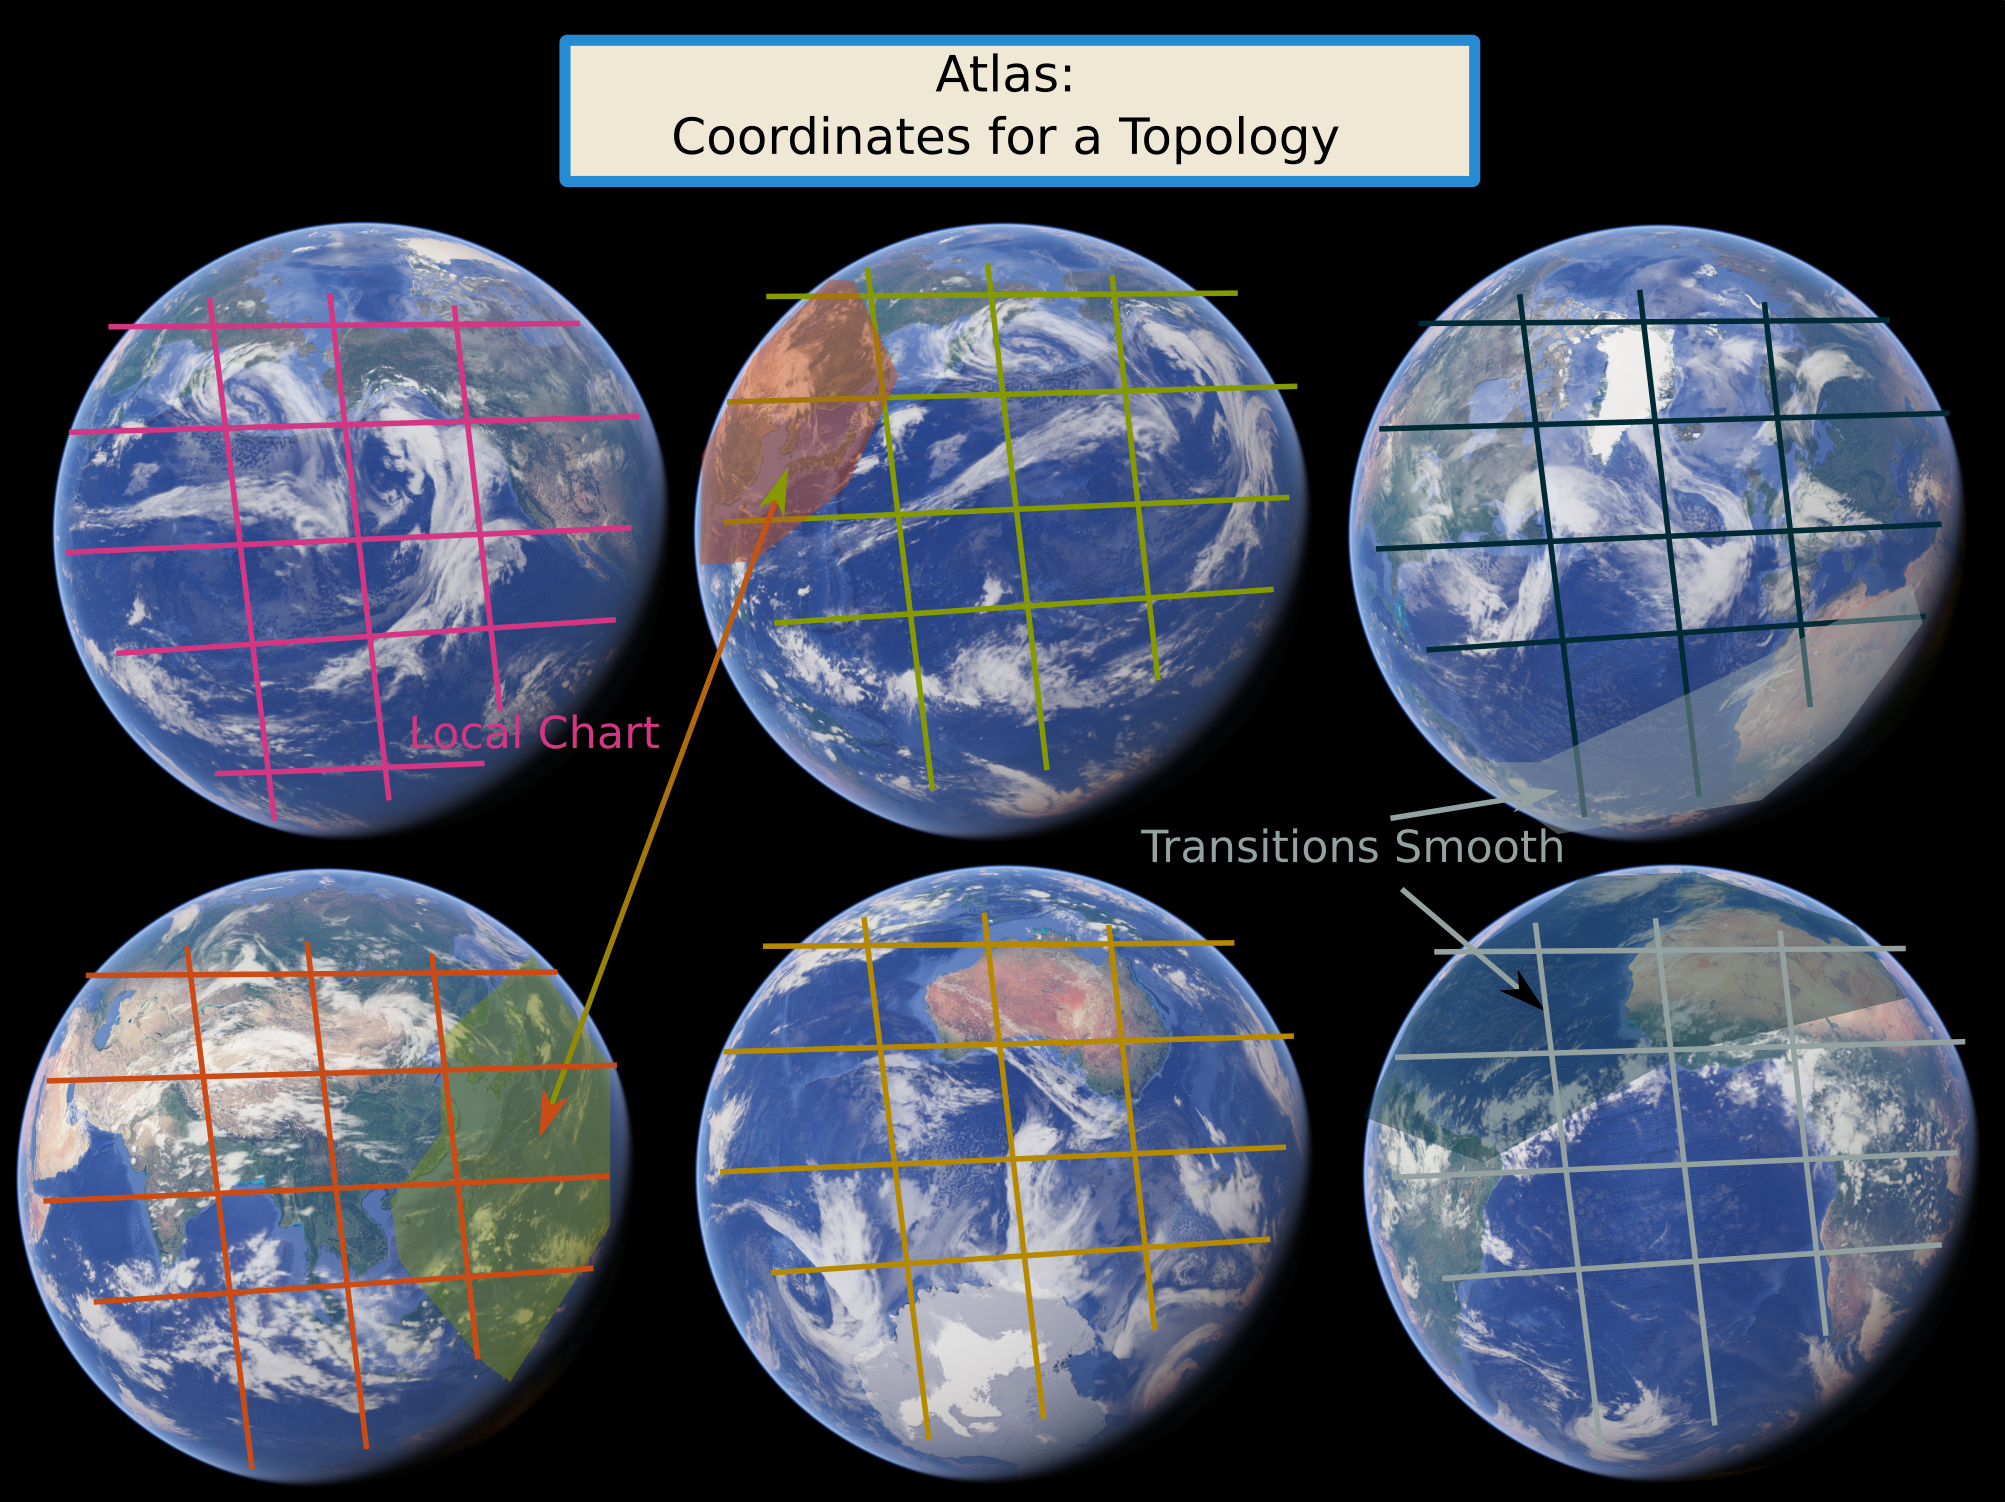
\includegraphics[width=\textwidth]{pics/atlas.png}
  \caption{An atlas is composed of sets which possess coordinate systems, and smooth transition functions between the coordinate systems where the sets overlap.}
    \label{fig:atlas}
\end{figure}

\include{Text/Homology}
\chapter{Homology}
\section{Simplicial Complexes}
An $n$-Simplex is an set of $(n+1)$ linearly independent points. We can think of them as $n$-dimensional generalizations of triangles.

For some low dimensional examples,
\begin{center}
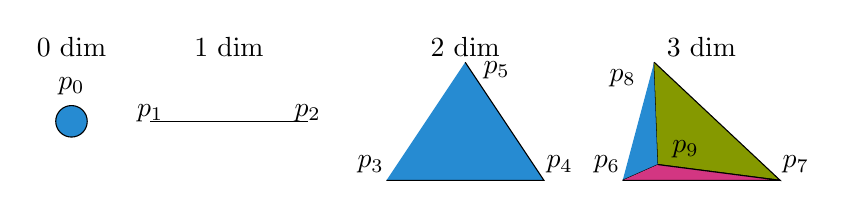
\begin{tikzpicture}
  \draw[fill=blue] (0,.75) circle (0.2);
  \draw (0,1.2) node{ $p_0$};
  \draw (0,1.7) node{0 dim};

  \draw (1,.75) -- (3,.75);
  \draw (1,.85) node{$p_1$};
  \draw (3,.85) node{$p_2$};
  \draw (2,1.7) node{1 dim};

  \draw[fill=blue] (4,0) -- (6,0) -- (5,1.5);
  \draw (3.8,.2) node{$p_3$};
  \draw (6.2,.2) node{$p_4$};
  \draw (5.4,1.4) node{$p_5$};
  \draw (5,1.7) node{2 dim};

  \draw[fill=blue] (7,0) -- (7.45,.2) -- (7.4,1.5);
  \draw[fill=green] (7.45,.2) -- (9,0) -- (7.4,1.5);
  \draw[fill=magenta] (7,0) -- (9,0) -- (7.45,.2);
  \draw (6.8,.2) node{$p_6$};
  \draw (9.2,.2) node{$p_7$};
  \draw (7,1.3) node{$p_8$};
  \draw (7.8,.4) node{$p_9$};
  \draw (8,1.7) node{3 dim};

\end{tikzpicture}
\end{center}

Both unoriented and oriented simplices exist.  For our purposes, we will be using oriented simplices.  The orientation is a positive or negative sign associated with the set.  Permuting the order of the points in the set can change the orientation.
\begin{equation}
  p_1 p_2 = - p_2 p_1 \qquad \qquad p_3 p_4 p_5 = - p_4 p_3 p_5 = p_5 p_3 p_4
\end{equation}
\begin{center}
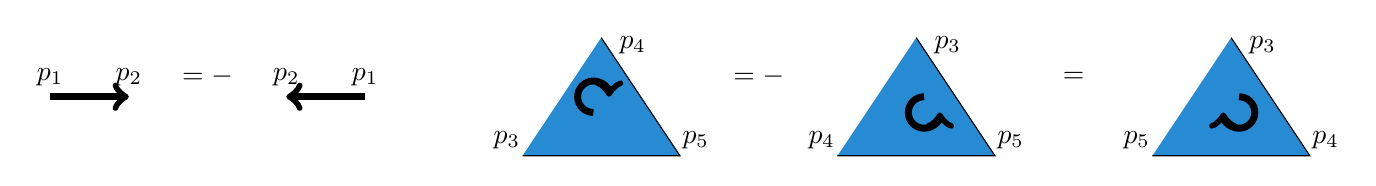
\begin{tikzpicture}
  \draw[->,line width=2.5] (1,.75) -- (2,.75);
  \draw (1,1) node{$p_1$};
  \draw (2,1) node{$p_2$};

  \draw (3,1) node{$=-$};

  \draw[<-,line width=2.5] (4,.75) -- (5,.75);
  \draw (4,1) node{$p_2$};
  \draw (5,1) node{$p_1$};


  \draw[fill=blue] (7,0) -- (9,0) -- (8,1.5);
  \draw (6.8,.2) node{$p_3$};
  \draw (9.2,.2) node{$p_5$};
  \draw (8.4,1.4) node{$p_4$};
  \draw[line width=2.5,<-] (8.1,.75) arc(0:270:.2);

  \draw (10,1) node{$=-$};

  \draw[fill=blue] (11,0) -- (13,0) -- (12,1.5);
  \draw (10.8,.2) node{$p_4$};
  \draw (13.2,.2) node{$p_5$};
  \draw (12.4,1.4) node{$p_3$};
  \draw[line width=2.5,->] (12.1,.75) arc(90:360:.2);

  \draw (14,1) node{$=$};

  \draw[fill=blue] (15,0) -- (17,0) -- (16,1.5);
  \draw (14.8,.2) node{$p_5$};
  \draw (17.2,.2) node{$p_4$};
  \draw (16.4,1.4) node{$p_3$};
  \draw[line width=2.5,->] (16.1,.75) arc(90:-180:.2);

\end{tikzpicture}
\end{center}
While we can see direction in one and two dimensions, this concept is trickier to conceptualize in higher dimensions.  In higher dimensions, instead of thinking pictorially, we need to just think in terms of even or odd permutations of an ordered set.
\begin{equation}
  p_1 p_2 p_3 p_4 p_5 = - (p_2 p_1) p_3 p_4 p_5
\end{equation}

By adding multiple simplices of the same dimension together, we can form a \textbf{chain}.  For example, this is a 2-chain,
\begin{equation}
  p_1 p_2 p_2 + p_2 p_3 p_4
\end{equation}
\begin{center}
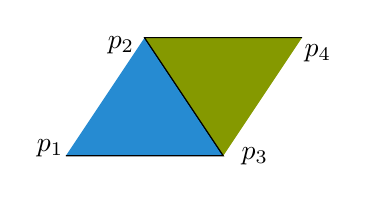
\begin{tikzpicture}
  \draw (-.2,.1) node{$p_1$};
  \draw (.7,1.4) node{$p_2$};
  \draw (2.4,0) node{$p_3$};
  \draw (3.2,1.3) node{$p_4$};

  \draw[fill=blue] (0,0) -- (2,0) -- (1,1.5);
  \draw[fill=green] (2,0) -- (1,1.5) -- (3,1.5);
\end{tikzpicture}
\end{center}

Each simplex gives us a collection of points.  From that collection of points, we can decide to just choose a subset of those and look at those instead.  This subset is a \textbf{face} of the simplex.  For example, if we look at the three dimensional simplex above, $p_6 p_7 p_8 p_9$, we could choose the 2-face $p_6 p_7 p_8$.  All the faces make up the boundaries and edges of an object. We should be able to determine things about the boundaries of an object that are independent of the particular way we write in down but just dependent on the global, qualitative features of the object.  This will show up in how an object relates to its faces.

To study how an object relates to its faces, we need to introduce a boundary operator  $ \partial: \sigma_n \rightarrow \sigma_{n-1} $
\begin{tcolorbox}
\begin{equation}
  \partial \left(p_1 \dots p_n \right)
  = \sum_{i=1}^n (-1)^{i} p_1 \dots \hat{p_i} \dots p_n
\end{equation}
\end{tcolorbox}
where $\hat{p_i}$ is omitted.  For example,
\begin{align}
  \partial(p_0) &= 0 \\
  \partial(p_1 p_2) & = p_2 - p_1 \\
  \partial(p_1 p_2 p_3) & = -p_2 p_3 + p_1 p_3 - p_1 p_2
\end{align}
The boundary of a boundary is always zero,
\begin{tcolorbox}
  \begin{equation}\label{eq:boundary_zero}
    \partial \partial \sigma =0.
  \end{equation}
\end{tcolorbox}
We can verify this for the boundaries just calculated,
\begin{align}
  \partial \partial (p_0 )& = \partial 0  &= 0 \\
  \partial \partial (p_1 p_2 )&= \partial (p_2 - p_1) &= 0 \\
  \partial \partial (p_1 p_2 p_3 )&= \partial (-p_2 p_3 + p_1 p_3 - p_1 p_2) &=
    p_2 - p_3 -p_1 + p_3  + p_1 -p_2 =0 ,
\end{align}
or in general for any dimension.





\begin{definition}[Simplicial Complex]
  A simplicial complex is a set of of simplices $\kappa$ such that
  \begin{itemize}
    \item For every simplex $\sigma \in \kappa$, every face of the simplex is also in $\kappa$
    \item The intersection of two simplices is a face of both simplices, $\sigma_1 \cap \sigma_2 \in \sigma_1 , \sigma_2$
  \end{itemize}
\end{definition}

For example,
\begin{center}
  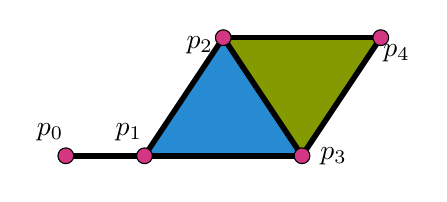
\begin{tikzpicture}

    \draw[fill=blue] (0,0) -- (2,0) -- (1,1.5);
    \draw[fill=green] (2,0) -- (1,1.5) -- (3,1.5);

    \draw[line width=2] (0,0) -- (-1,0);
    \draw[line width=2] (0,0) -- (1,1.5);
    \draw[line width=2] (0,0) -- (2,0);
    \draw[line width=2] (2,0) -- (1,1.5);
    \draw[line width=2] (1,1.5) -- (3,1.5);
    \draw[line width=2] (2,0) -- (3,1.5);

    \draw  (-1.2,.3) node{$p_0$};
    \draw[fill=magenta] (-1,0) circle (0.1);
    \draw (-.2,.3) node{$p_1$};
    \draw[fill=magenta] (0,0) circle (0.1);
    \draw (.7,1.4) node{$p_2$};
    \draw[fill=magenta] (1,1.5) circle (0.1);
    \draw (2.4,0) node{$p_3$};
    \draw[fill=magenta] (2,0) circle (0.1);
    \draw (3.2,1.3) node{$p_4$};
    \draw[fill=magenta] (3,1.5) circle (0.1);

  \end{tikzpicture}
\begin{tabular}{c c c}
  \hline
  dim 0 & dim 1 & dim 2 \\
  \hline
  $p_0$ & $p_0 p_1$ & $p_1 p_2 p_3 $ \\
  $p_1$ & $p_1 p_2$ & $p_2 p_3 p_4 $ \\
  $p_2$ & $p_2 p_3$ & \\
  $p_3$ & $p_3 p_4$ & \\
  $p_4$ & $p_4 p_2$ & \\
   & $p_1 p_3$ & \\
   \hline
\end{tabular}
\end{center}
is a simplicial complex.  If we take the intersection of the simplices $p_1 p_2 p_3$ and $p_2 p_3 p_4$, we get $p_2 p_3$, which is a face of both simplices and in the simplicial complex.

But
\begin{center}
  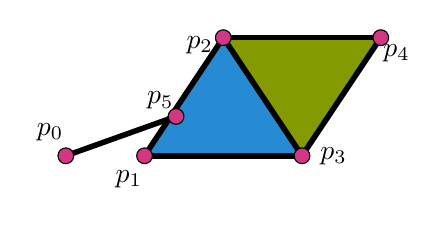
\begin{tikzpicture}

    \draw[fill=blue] (0,0) -- (2,0) -- (1,1.5);
    \draw[fill=green] (2,0) -- (1,1.5) -- (3,1.5);

    \draw[line width=2] (.4,.5) -- (-1,0);

    \draw[line width=2] (0,0) -- (2,0);
    \draw[line width=2] (0,0) -- (1,1.5);
    \draw[line width=2] (2,0) -- (1,1.5);
    \draw[line width=2] (1,1.5) -- (3,1.5);
    \draw[line width=2] (2,0) -- (3,1.5);


    \draw  (-1.2,.3) node{$p_0$};
    \draw[fill=magenta] (-1,0) circle (0.1);
    \draw (-.2,-.3) node{$p_1$};
    \draw[fill=magenta] (0,0) circle (0.1);
    \draw (.7,1.4) node{$p_2$};
    \draw[fill=magenta] (1,1.5) circle (0.1);
    \draw (2.4,0) node{$p_3$};
    \draw[fill=magenta] (2,0) circle (0.1);
    \draw (3.2,1.3) node{$p_4$};
    \draw[fill=magenta] (3,1.5) circle (0.1);

    \draw (.2,.7) node{$p_5$};
    \draw[fill=magenta] (.4,.5) circle (0.1);
  \end{tikzpicture}
\end{center}
is not a simplicial complex.  What even is the intersection of $p_0 p_5$ and $p_1 p_2$?  It's certainly not a face of either simplex.

The simplicial complex
\begin{center}
  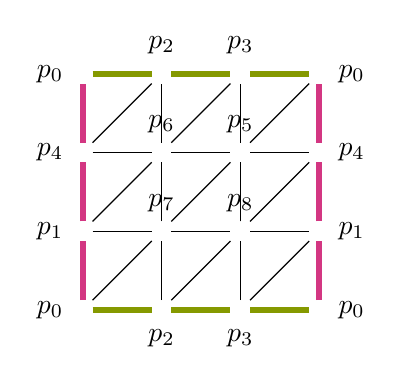
\begin{tikzpicture}
    \node (p0) at (0,0) [label=left:$p_0$]{};
    \node (p1) at (0,1) [label=left:$p_1$]{};
    \node (p2) at (1,0) [label=below:$p_2$]{};
    \node (p3) at (2,0) [label=below:$p_3$]{};
    \node (p4) at (0,2) [label=left:$p_4$]{};

    \node (p7) at (1,1) [label=above:$p_7$]{};
    \node (p8) at (2,1) [label=$p_8$]{};
    \node (p5) at (2,2) [label=$p_5$]{};
    \node (p6) at (1,2) [label=$p_6$]{};

    \node (p0p) at (3,0) [label=right:$p_0$]{};
    \node (p0ppp) at (3,3) [label=right:$p_0$]{};
    \node (p0pp) at (0,3) [label=left:$p_0$]{};
    \node (p1p) at (3,1) [label=right:$p_1$]{};
    \node (p2p) at (1,3) [label=above:$p_2$]{};
    \node (p3p) at (2,3) [label=above:$p_3$]{};
    \node (p4p) at (3,2) [label=right:$p_4$]{};

     \draw[magenta, line width = 2] (p0) -- (p1);
     \draw[magenta, line width = 2] (p0p) -- (p1p);
     \draw[magenta, line width = 2] (p1) -- (p4);
     \draw[magenta, line width = 2] (p1p) -- (p4p);
     \draw[magenta, line width = 2] (p4) -- (p0pp);
     \draw[magenta, line width = 2] (p4p) -- (p0ppp);

     \draw[green, line width = 2] (p0) -- (p2);
     \draw[green, line width = 2] (p2) -- (p3);
     \draw[green, line width = 2] (p3) -- (p0p);
     \draw[green, line width = 2] (p0pp) -- (p2p);
     \draw[green, line width = 2] (p2p) -- (p3p);
     \draw[green, line width = 2] (p3p) -- (p0ppp);

     \draw (p1) -- (p7);
     \draw (p0) -- (p7);
     \draw (p2) -- (p7);

     \draw (p2) -- (p8);
     \draw (p7) -- (p8);
     \draw (p3) -- (p8);

     \draw (p3) -- (p1p);
     \draw (p8) -- (p1p);
     \draw (p8) -- (p4p);
     \draw (p8) -- (p5);

     \draw (p1) -- (p6);
     \draw (p4) -- (p6);
     \draw (p7) -- (p6);

     \draw (p6) -- (p5);
     \draw (p7) -- (p5);
     \draw (p8) -- (p5);

     \draw (p5) -- (p4p);
     \draw (p5) -- (p0ppp);
     \draw (p5) -- (p3p);

     \draw (p6) -- (p3p);
     \draw (p6) -- (p2p);
     \draw (p4) -- (p2p);

  \end{tikzpicture}
\end{center}
is equivalent to a torus.  You can see that that edges are in fact the same points.  Since I couldn't figure out how to perform this manipulation with computer graphics, here's the manipulation with good, old fashioned arts and crafts,

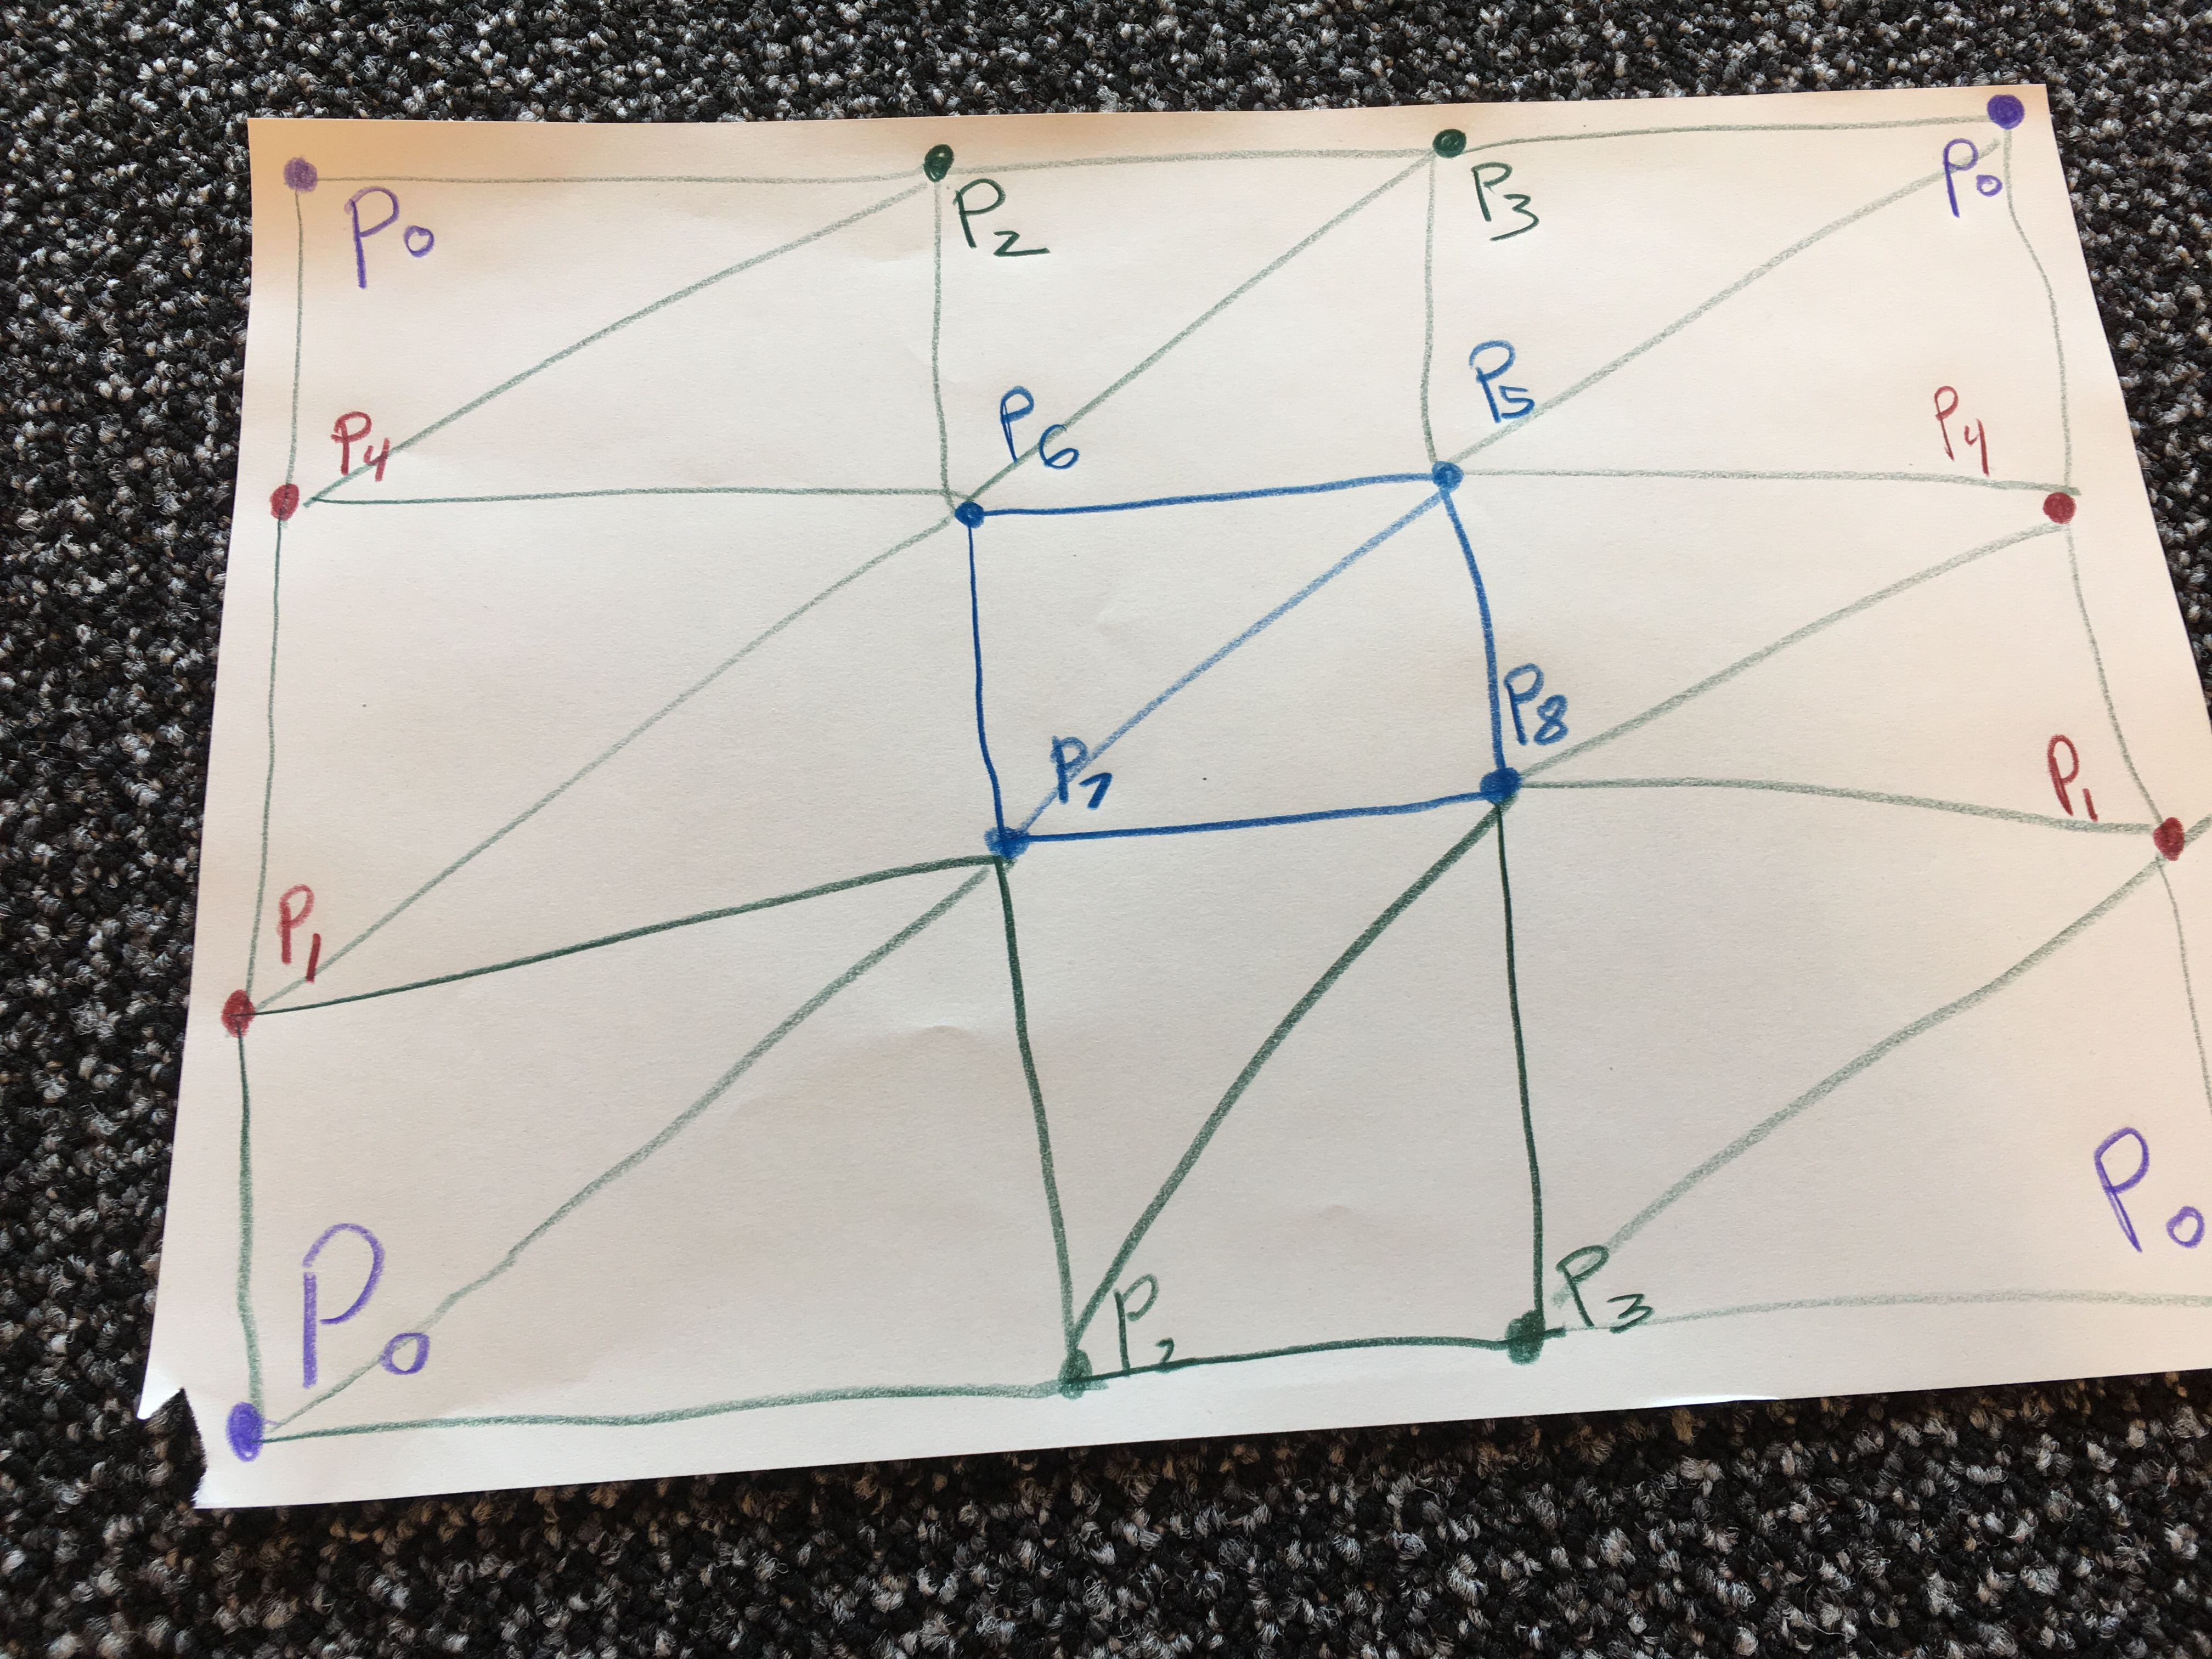
\includegraphics[width=.25\textwidth]{pics/flat_torus.JPG}
{\fontsize{50}{60}\selectfont $\rightarrow$}
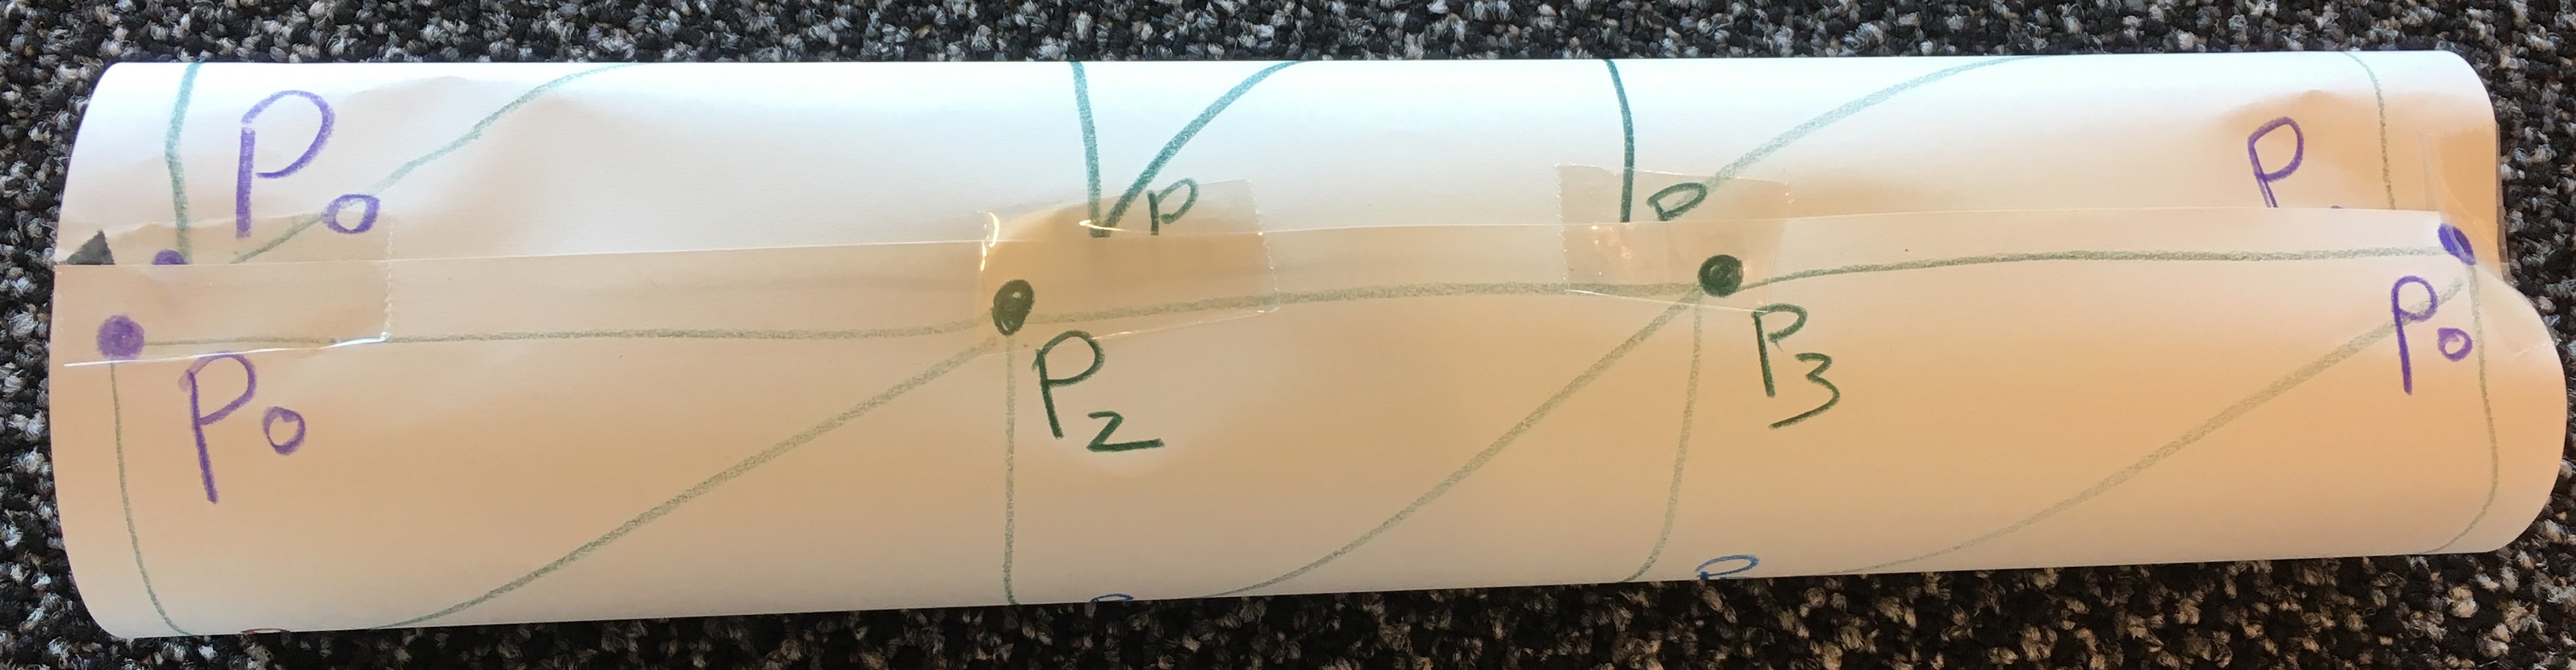
\includegraphics[width=.25\textwidth]{pics/torus_1curl.JPG}
{\fontsize{50}{60}\selectfont $\rightarrow$}
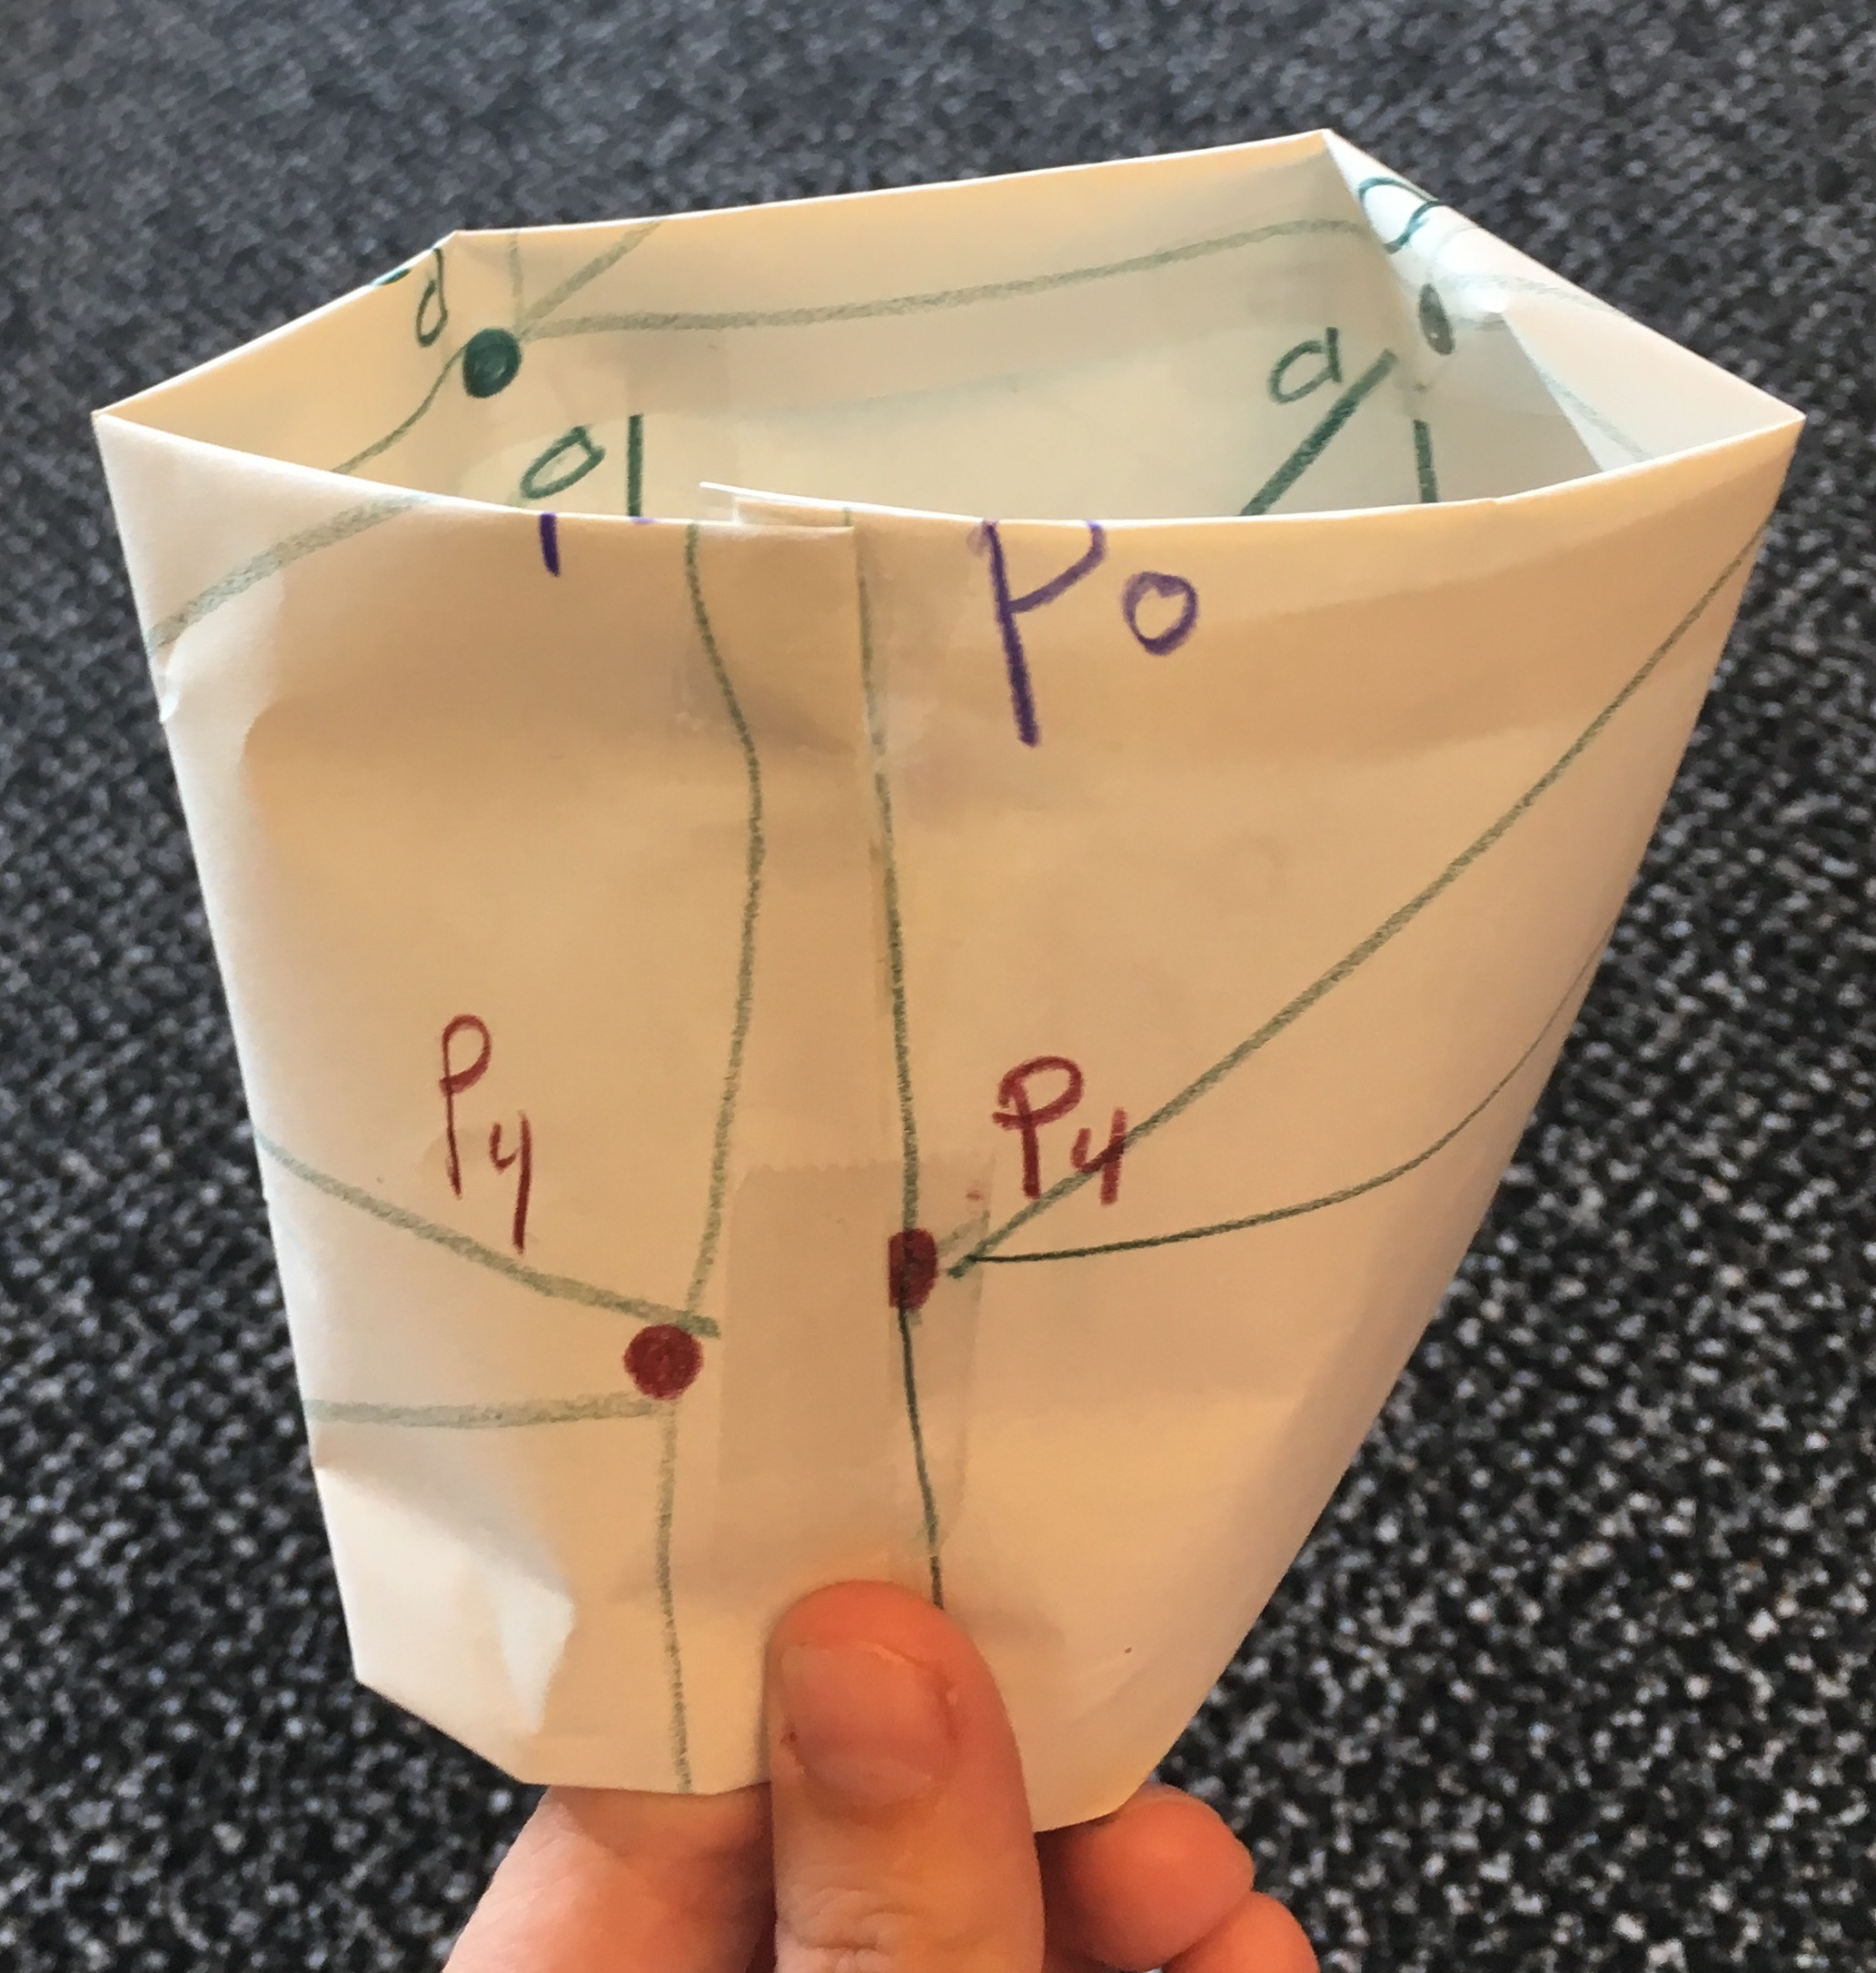
\includegraphics[width=.25\textwidth]{pics/torus_2curl.JPG}

I'll often use this simplicial complex as it's relatively simple, yet it still has some interesting structure.

\subsection{The group of cycles and the group of boundaries}

Let's take a chain.  For example,
\begin{equation}
\sigma_1=  p_7 p_6 + p_6 p_5 + p_5 p_7
\end{equation}
in the torus.  Two things about this chain are relevantly interesting to us.  First,
\begin{equation}
  \partial \sigma_1 = 0.
\end{equation}
The boundary of the chain is zero.  You can verify this for yourself.  Second,
\begin{equation}
  \exists \sigma_2 \qquad \text{such that} \qquad \partial \sigma_2 = \sigma_1.
\end{equation}
In particular, $\sigma_2 = p_7 p_6 p_5$, but that fact is not as important as the fact that \textit{it exists}.

The first property defines \textbf{Cycles}.
\begin{definition}[Cycle]
  A \textbf{Cycle} of dimension $d$ is a chain of dimension $d$ $\sigma$ in a simplicial complex such that $\partial \sigma =0$.
\end{definition}
We can add any two cycles of the same dimension together and get another cycle just because the boundary operator is distributive.  This means we have a group, particularly the group $Z_d (T)$, where $T$ is the given topology and $d$ is the dimension.

The second property defines \textbf{Boundaries}.
\begin{definition}[Boundary]
  If $\partial \sigma_2 = \sigma_1$ for some $\sigma_2$, then $\sigma_1$ is a \textbf{boundary}.
\end{definition}
 If a chain is the derivative of something else, then it is a boundary.  More formally, it's the image of the $\partial$ operator.  Boundaries of a certain dimension again will form a group $B_d (T)$, because of the distributivity of the boundary operator.

Since we know from eq~\ref{eq:boundary_zero} that the second derivative of every chain is zero, and every boundary is the derivative of a chain, then the derivative of every boundary is zero. Every boundary is then.... you guessed it... I hope, or I failed in explaining this ... a cycle.

\textbf{BUT} not every cycle is a boundary.

To see this, let us go back to our trusty torus and look at the cycle
\begin{equation}\label{eq:not_boundary}
  p_1 p_7 + p_7 p_8 + p_8 p_1.
\end{equation}
Go ahead an verify that this is indeed a cycle.  That is a rather straight forward calculation.  And then, waste some period of time trying to find a combination of simplices that will give that particular chain upon derivation.  Then give up and say it's impossible.  Physicist's proof.

You can think of every boundary being able to be continuously deformed to a point through the surface that it borders. But the chain~\ref{eq:not_boundary} can't be deformed away to a point because it wraps around the torus.  Only cutting and gluing the torus would allow you to deform that cycle down into a point.

  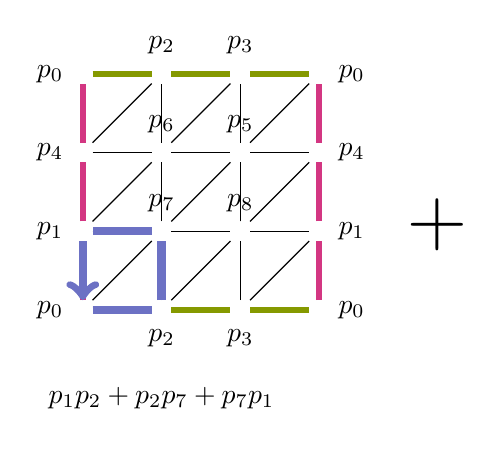
\begin{tikzpicture}
    \node (p0) at (0,0) [label=left:$p_0$]{};
    \node (p1) at (0,1) [label=left:$p_1$]{};
    \node (p2) at (1,0) [label=below:$p_2$]{};
    \node (p3) at (2,0) [label=below:$p_3$]{};
    \node (p4) at (0,2) [label=left:$p_4$]{};

    \node (p7) at (1,1) [label=above:$p_7$]{};
    \node (p8) at (2,1) [label=$p_8$]{};
    \node (p5) at (2,2) [label=$p_5$]{};
    \node (p6) at (1,2) [label=$p_6$]{};

    \node (p0p) at (3,0) [label=right:$p_0$]{};
    \node (p0ppp) at (3,3) [label=right:$p_0$]{};
    \node (p0pp) at (0,3) [label=left:$p_0$]{};
    \node (p1p) at (3,1) [label=right:$p_1$]{};
    \node (p2p) at (1,3) [label=above:$p_2$]{};
    \node (p3p) at (2,3) [label=above:$p_3$]{};
    \node (p4p) at (3,2) [label=right:$p_4$]{};

     \draw[magenta, line width = 2] (p0) -- (p1);
     \draw[magenta, line width = 2] (p0p) -- (p1p);
     \draw[magenta, line width = 2] (p1) -- (p4);
     \draw[magenta, line width = 2] (p1p) -- (p4p);
     \draw[magenta, line width = 2] (p4) -- (p0pp);
     \draw[magenta, line width = 2] (p4p) -- (p0ppp);

     \draw[green, line width = 2] (p0) -- (p2);
     \draw[green, line width = 2] (p2) -- (p3);
     \draw[green, line width = 2] (p3) -- (p0p);
     \draw[green, line width = 2] (p0pp) -- (p2p);
     \draw[green, line width = 2] (p2p) -- (p3p);
     \draw[green, line width = 2] (p3p) -- (p0ppp);

     \draw (p1) -- (p7);
     \draw (p0) -- (p7);
     \draw (p2) -- (p7);

     \draw (p2) -- (p8);
     \draw (p7) -- (p8);
     \draw (p3) -- (p8);

     \draw (p3) -- (p1p);
     \draw (p8) -- (p1p);
     \draw (p8) -- (p4p);
     \draw (p8) -- (p5);

     \draw (p1) -- (p6);
     \draw (p4) -- (p6);
     \draw (p7) -- (p6);

     \draw (p6) -- (p5);
     \draw (p7) -- (p5);
     \draw (p8) -- (p5);

     \draw (p5) -- (p4p);
     \draw (p5) -- (p0ppp);
     \draw (p5) -- (p3p);

     \draw (p6) -- (p3p);
     \draw (p6) -- (p2p);
     \draw (p4) -- (p2p);

     \draw[violet, line width=3, ->] (p0) -- (p2) -- (p7) -- (p1) -- (p0);

     \node (text) at (4.5,.5) [label={\fontsize{30}{40}\selectfont$+$}]{};
     \draw (text);

     \node (name) at (1,-1.5) [label=$p_1 p_2+p_2 p_7 + p_7 p_1$]{};
     \draw (text);
  \end{tikzpicture}
  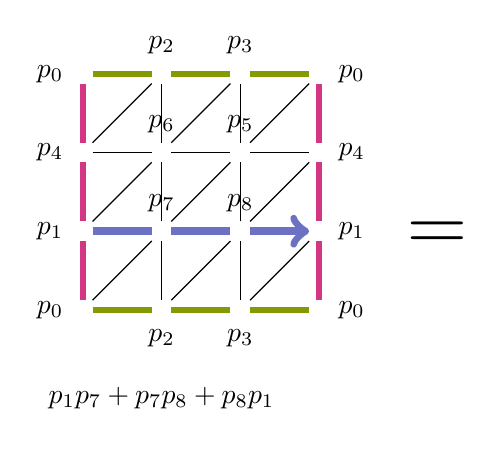
\begin{tikzpicture}
    \node (p0) at (0,0) [label=left:$p_0$]{};
    \node (p1) at (0,1) [label=left:$p_1$]{};
    \node (p2) at (1,0) [label=below:$p_2$]{};
    \node (p3) at (2,0) [label=below:$p_3$]{};
    \node (p4) at (0,2) [label=left:$p_4$]{};

    \node (p7) at (1,1) [label=above:$p_7$]{};
    \node (p8) at (2,1) [label=$p_8$]{};
    \node (p5) at (2,2) [label=$p_5$]{};
    \node (p6) at (1,2) [label=$p_6$]{};

    \node (p0p) at (3,0) [label=right:$p_0$]{};
    \node (p0ppp) at (3,3) [label=right:$p_0$]{};
    \node (p0pp) at (0,3) [label=left:$p_0$]{};
    \node (p1p) at (3,1) [label=right:$p_1$]{};
    \node (p2p) at (1,3) [label=above:$p_2$]{};
    \node (p3p) at (2,3) [label=above:$p_3$]{};
    \node (p4p) at (3,2) [label=right:$p_4$]{};

     \draw[magenta, line width = 2] (p0) -- (p1);
     \draw[magenta, line width = 2] (p0p) -- (p1p);
     \draw[magenta, line width = 2] (p1) -- (p4);
     \draw[magenta, line width = 2] (p1p) -- (p4p);
     \draw[magenta, line width = 2] (p4) -- (p0pp);
     \draw[magenta, line width = 2] (p4p) -- (p0ppp);

     \draw[green, line width = 2] (p0) -- (p2);
     \draw[green, line width = 2] (p2) -- (p3);
     \draw[green, line width = 2] (p3) -- (p0p);
     \draw[green, line width = 2] (p0pp) -- (p2p);
     \draw[green, line width = 2] (p2p) -- (p3p);
     \draw[green, line width = 2] (p3p) -- (p0ppp);

     \draw (p1) -- (p7);
     \draw (p0) -- (p7);
     \draw (p2) -- (p7);

     \draw (p2) -- (p8);
     \draw (p7) -- (p8);
     \draw (p3) -- (p8);

     \draw (p3) -- (p1p);
     \draw (p8) -- (p1p);
     \draw (p8) -- (p4p);
     \draw (p8) -- (p5);

     \draw (p1) -- (p6);
     \draw (p4) -- (p6);
     \draw (p7) -- (p6);

     \draw (p6) -- (p5);
     \draw (p7) -- (p5);
     \draw (p8) -- (p5);

     \draw (p5) -- (p4p);
     \draw (p5) -- (p0ppp);
     \draw (p5) -- (p3p);

     \draw (p6) -- (p3p);
     \draw (p6) -- (p2p);
     \draw (p4) -- (p2p);

     \draw[violet, line width=3, ->] (p1) -- (p7) -- (p8)  -- (p1p);

     \node (text) at (4.5,.5) [label={\fontsize{30}{40}\selectfont$=$}]{};
     \draw (text);

     \node (name) at (1,-1.5) [label=$p_1 p_7 + p_7 p_8 + p_8 p_1$]{};
     \draw (text);
  \end{tikzpicture}
  \begin{tikzpicture}
    \node (p0) at (0,0) [label=left:$p_0$]{};
    \node (p1) at (0,1) [label=left:$p_1$]{};
    \node (p2) at (1,0) [label=below:$p_2$]{};
    \node (p3) at (2,0) [label=below:$p_3$]{};
    \node (p4) at (0,2) [label=left:$p_4$]{};

    \node (p7) at (1,1) [label=above:$p_7$]{};
    \node (p8) at (2,1) [label=$p_8$]{};
    \node (p5) at (2,2) [label=$p_5$]{};
    \node (p6) at (1,2) [label=$p_6$]{};

    \node (p0p) at (3,0) [label=right:$p_0$]{};
    \node (p0ppp) at (3,3) [label=right:$p_0$]{};
    \node (p0pp) at (0,3) [label=left:$p_0$]{};
    \node (p1p) at (3,1) [label=right:$p_1$]{};
    \node (p2p) at (1,3) [label=above:$p_2$]{};
    \node (p3p) at (2,3) [label=above:$p_3$]{};
    \node (p4p) at (3,2) [label=right:$p_4$]{};

     \draw[magenta, line width = 2] (p0) -- (p1);
     \draw[magenta, line width = 2] (p0p) -- (p1p);
     \draw[magenta, line width = 2] (p1) -- (p4);
     \draw[magenta, line width = 2] (p1p) -- (p4p);
     \draw[magenta, line width = 2] (p4) -- (p0pp);
     \draw[magenta, line width = 2] (p4p) -- (p0ppp);

     \draw[green, line width = 2] (p0) -- (p2);
     \draw[green, line width = 2] (p2) -- (p3);
     \draw[green, line width = 2] (p3) -- (p0p);
     \draw[green, line width = 2] (p0pp) -- (p2p);
     \draw[green, line width = 2] (p2p) -- (p3p);
     \draw[green, line width = 2] (p3p) -- (p0ppp);

     \draw (p1) -- (p7);
     \draw (p0) -- (p7);
     \draw (p2) -- (p7);

     \draw (p2) -- (p8);
     \draw (p7) -- (p8);
     \draw (p3) -- (p8);

     \draw (p3) -- (p1p);
     \draw (p8) -- (p1p);
     \draw (p8) -- (p4p);
     \draw (p8) -- (p5);

     \draw (p1) -- (p6);
     \draw (p4) -- (p6);
     \draw (p7) -- (p6);

     \draw (p6) -- (p5);
     \draw (p7) -- (p5);
     \draw (p8) -- (p5);

     \draw (p5) -- (p4p);
     \draw (p5) -- (p0ppp);
     \draw (p5) -- (p3p);

     \draw (p6) -- (p3p);
     \draw (p6) -- (p2p);
     \draw (p4) -- (p2p);

     \draw[violet, line width=3, ->] (p1) -- (p0) -- (p2) -- (p7) -- (p8) -- (p1p);

     \node (name) at (1,-1.5) [label=$p_1 p_0 + p_0 p_2 + p_0 p_7 + p_7 p_8 + p_8 p_1$]{};
     \draw (text);
  \end{tikzpicture}



  \begin{equation}
    \left( p_1 p_2+p_2 p_7 + \cancel{p_7 p_1} \right) + \left( \cancel{p_1 p_7} + p_7 p_8 + p_8 p_1 \right)
  \end{equation}


  \begin{equation}
    \partial \left( p_7 p_0 p_1 + p_2 p_0 p_7 \right)
    =  - p_0 p_1 + p_7 p_1 - \cancel{p_7 p_0} - \cancel{p_0 p_7} + p_2 p_7 - p_2 p_0
    = p_0 p_2 + p_2 p_7 + p_7 p_1 + p_1 p_0
  \end{equation}

\chapter{Differential Calculus}

Suppose we have a path $\vec{f}(t)$ on a manifold $M$.  For a neighborhood $U$ with a coordinate system $(x_1, x_2,..., x_n)$ around a point $p(t_0)$.  Using the chain rule around this point,
\begin{align}
  \d{f}{t} & = \pd{f}{x_1}\pd{x_1}{t} + \pd{f}{x_2}\pd{x_2}{t} + ... + \pd{f}{x_n} \pd{x_n}{t} \\
  & = \left(v^1 \pd{}{x_1} + v^2 \pd{}{x_2} + ... + v^n \pd{}{x_n} \right) f
\end{align}
Using all functions through the point, we can construct a vector space that acts as an operator on functions.  The vector space has components $(v^1, v^2, ..., v^n)$ and a basis $(\pd{}{x_1}, \pd{}{x_2},...,\pd{}{x_n})$.  The set of all such objects created by all functions through point $p(t_0)$ is the \textbf{Tangent Space} $TM(p(t_0))$ at point $p(t_0)$.  When we take the set of all the tangent spaces at all the points on the manifold, we get the \textbf{Tangent Bundle} $TM$.  More about bundles in the next section.

Under a change of basis $ \vec{x} \rightarrow \vec{y}(\vec{x} ) $, the bases change \textbf{covariantly} as
\begin{equation}
  \mathbf{e}^y_i = \pd{}{y_i} = \sum_j \pd{x_j}{y_i}\pd{}{x_j} = \sum_j \pd{x_j}{y_i} \mathbf{e}^x_j = \sum_j  R^j_i \mathbf{e}^x_j \qquad \qquad R^j_i = \pd{x_j}{y_i}.
\end{equation}
The vector components, $v^i$, on the other hand, transform \textbf{contravariantly} as
\begin{equation}
  v^i_y = \pd{y_i}{t} = \sum_j \pd{y_i}{x_j} \pd{x_j}{t} = \sum_j \pd{y_i}{x_j} v^j_x
  = \sum_j \left(R^{-1} \right)^i_j v_x^j \qquad \qquad \left(R^{-1}\right)^i_j = \pd{y_i}{x_j}
\end{equation}
Indeed $R$ and $R^{-1}$ are inverses as
\begin{equation}
 R^i_j (R^{-1})^j_i = \pd{x_i}{y_j} \pd{y_j}{x_i} = \delta_{i,j}
\end{equation}

Now the terminology of this can get very confusing; remembering which objects are contravariant or covariant, which transformations are covariant and which are contravariant, etc. The names really don't matter as much as understanding that you need one of each to create a geometrically invariant quantity.  You can determine what goes on top and bottom of a transformation matrix by simply applying the chain rule each time.  Just remember what that $\mathbf{e}_i$ stands for $\pd{}{x_i}$, and you can work everything out from there, without getting hung up on vocabulary.


We can think of the contravariant components acting on the covariant bases and spitting out a basis independent object, $\d{f}{t}$.
\begin{equation}
  v: \mathbf{e} \rightarrow \d{f}{t}   \qquad \qquad
  \text{contravariant} :  \text{covariant}  \rightarrow \text{invariant}
\end{equation}
Conversely, we could also write
\begin{equation}
\mathbf{e} : v \rightarrow \d{f}{t} \qquad \qquad \text{convariant} : \text{contravariant} \rightarrow \text{invariant}
\end{equation}
In this way, we have been writing out bases as the covariant objects, but we could also construct a \textbf{covector} space \textbf{dual} to the vector space we just constructed, where instead the bases are contravariant and the components are covariant.

\begin{table}
  \center
  \def\arraystretch{1.5}
  \begin{tabular}{| c | c | c |}
    \hline
    & Covariant &  Contravariant  \\
    \hline
    Tangent Space & bases $\mathbf{e}_i = \pd{}{x_i}$ & components $v^i$ \\
    Cotangent Space & components $v_i$ & bases $\omega^i = \text{d}x^i$ \\
    \hline
  \end{tabular}
  \caption{The transformation properties of vectors and covectors.}
  \label{tab:trans}
\end{table}

To construct the \textbf{Cotangent bundle} we can proceed analogously to our contruction of the Tangent bundle, but instead at a point $p$, we only look at
\begin{align}
  df & = \pd{f}{x_1} \text{d}x^1 + \pd{f}{x_2} \text{d}x^2 + ...
  + \pd{f}{x_n} \text{d}x^n \\
  & = v_1 \omega^1 + v_2 \omega^2 + ... + v_n \omega^n
\end{align}
For these objects we have the transformation properties
\begin{equation}
  v^y_i =\pd{f}{y_i} = \sum_j \pd{f}{x_j} \pd{x_j}{y_i} = \sum_j \pd{x_j}{y_i} v^x_j = \sum_j R^j_i v^x_j
\end{equation}
\begin{equation}
  \omega^i_y = \text{d}y^i = \sum_j \pd{y^i}{x_j} \text{d}x^j =
  \sum_j \pd{y^i}{x_j} \omega^j_x = \sum_j (R^{-1})^i_j \omega^j_x
\end{equation}

\chapter{Vector Bundles}

\begin{definition}[Fiber Bundle]
A \textbf{Fiber Bundle} is a topological space $E$, a manifold $M$, and a function $\pi : E \rightarrow M$, where the \textbf{Fiber} $F$ for a point $p \in M$ is $\pi^{-1} (p)$. In order for the set to be a Fiber Bundle, any neighborhood $U$ of $p\in M$, $\pi^{-1}(U)$ is homomorphic to $U \times F$.
\end{definition}

\begin{example} \label{ex:r2} For example $E = \mathcal{R}^2$, $M=\mathcal{R}$, and $\pi: (x,y) \rightarrow x$. See Fig~\ref{fig:r2}
\end{example}

\begin{example} The Mobius strip is a non-trivial bundle where the $M=\mathcal{S}$ and the fiber is $\mathcal{R}$.  See Fig~\ref{fig:mobius}
\end{example}

\begin{figure}
  \begin{subfigure}{.4\textwidth}
  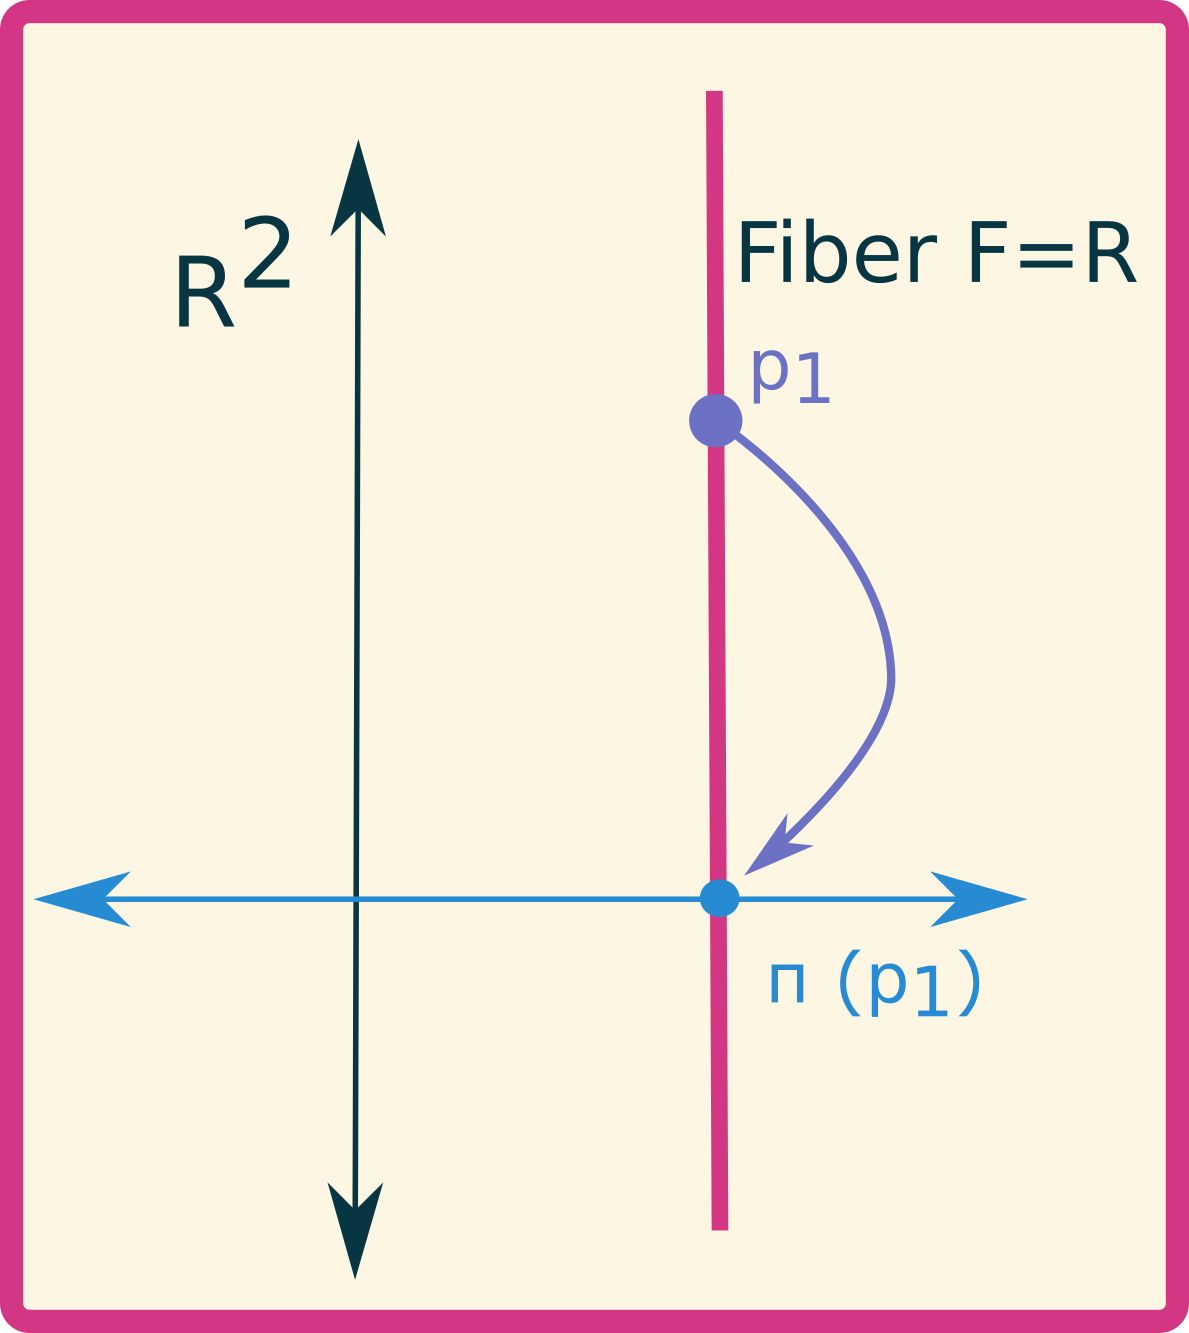
\includegraphics[width=\textwidth]{pics/r2.png}
  \caption{}
  \label{fig:r2}
\end{subfigure}
\begin{subfigure}{.6\textwidth}
  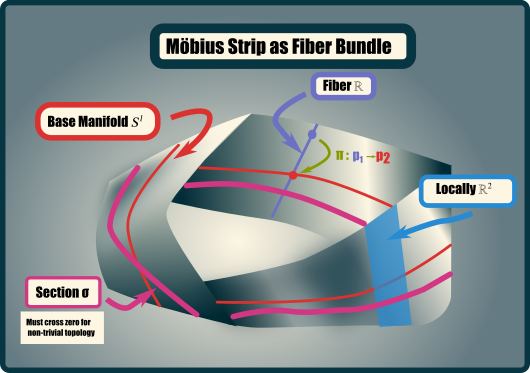
\includegraphics[width=\textwidth]{pics/mobius.png}
  \caption{}
  \label{fig:mobius}
\end{subfigure}
  \label{fig:fiberbundles}
  \caption{a) A simple fiber bundle. b) A Mobius strip is a simple non-trivial fiber bundle.}
\end{figure}

\begin{definition}[Section]
A \textbf{Section} is a function $\sigma : M \rightarrow E$ such that $\pi \cdot \sigma : M \rightarrow M$ is the identity map on $M$.
\end{definition}

\begin{example} Given our vector bundle from Example~\ref{ex:r2},  take the section $\sigma(x) = (x,x^2)$.  If we then apply the $\pi$ projection function, $\pi (x,x^2) = x$.  So our composition would be the identity and $\sigma$ is a valid section.
\end{example}

\section{Connections on Bundles}
Let's just look at a local neighborhood $U$ around point $p$ where we have a coordinate system $(x_0, x_1, ..., x_n)$ on our vector bundle of interest.  Given this coordinate system, we can create derivatives
\begin{equation}
  \text{d}f = \d{f}{x_0} \text{d}x_0 + \d{f}{x_1} \text{d}x_1 + ... + \d{f}{x_n} \text{d}x_n
\end{equation}
given some function $f$ through the point of interest $p$ in the neighborhood $U$. The vector $(\d{}{x_0}, \d{}{x_1},...,\d{}{x_n}) $ defines the \textbf{Tangent space}, and the covector $(\text{d} x_0, \text{d}x_1, ..., \text{d} x_n)$ defines the \textbf{Cotangent space} at point $p$.

The next step takes a bit of adjustment to understand.  We have to make a \textit{choice}.  Just like how we imposed extra structure on sets to create topologies, or on topologies to make bundles, we now have to impose extra structure on our bundle that does not intrinsically exist.  Without making this \textit{choice}, we actually do not have anyway to connect to fibers adjacent to each other on the same bundle.

  \begin{wrapfigure}{L}{.4\textwidth}\begin{center}
    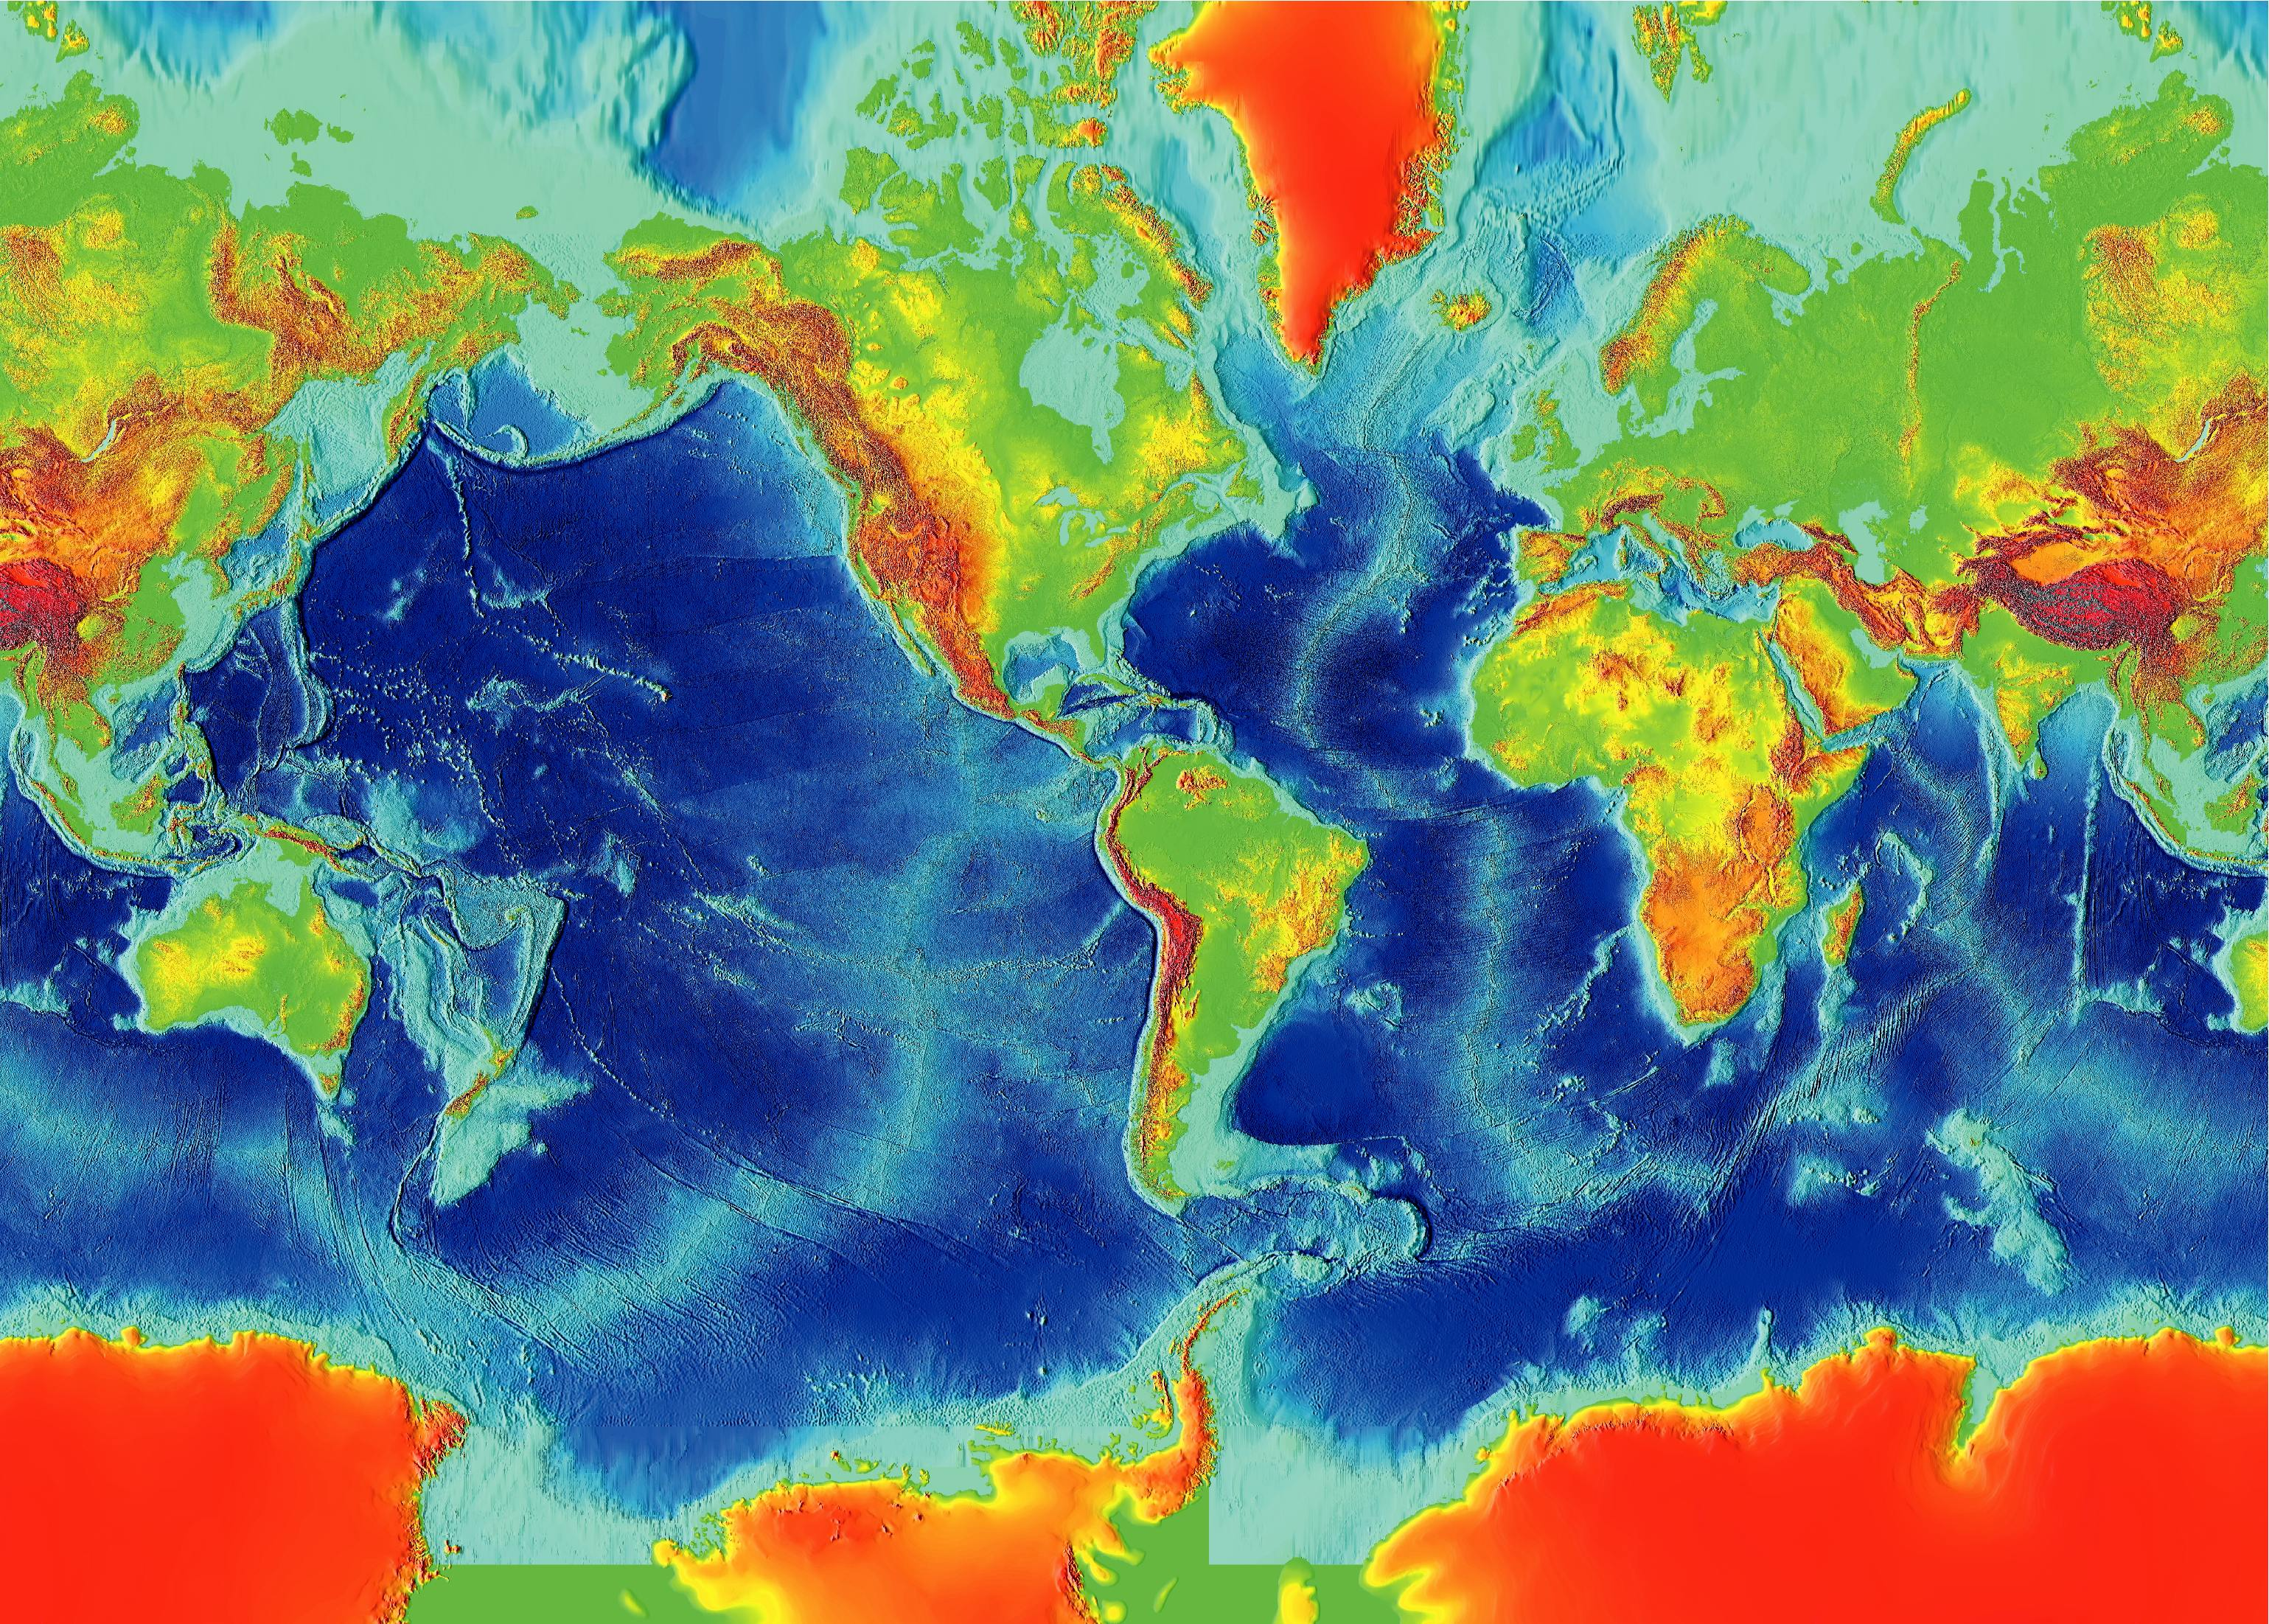
\includegraphics[width=.35\textwidth]{pics/earth_surface.jpg}\end{center}
    \caption{ \protect\footnotemark }
  \end{wrapfigure}
\footnotetext{File:Earth surface NGDC 2000.jpg|Earth surface NGDC 2000}

  Normally we describe the Earth as just a perfect sphere, $S^2$, but it's not.  So let us instead describe it as a fiber bundle where each point of the base manifold of $S^2$ has possible heights associated with it pulled from $\mathbb{R}$.  The surface of the Earth will be a section defined on the sphere. We can see those values in the elevation map to the right.

  Only after we define the surface of the Earth can we say what vectors go along the surface of the Earth, what vectors are perpendicular (complimentary to the surface) to the Earth, and how I would get to the top of Fuji-yama.  If I assumed the Earth was a perfect sphere, climbing Fuji-yama would land me deep in some pretty toxic substances.  I have to account for how moving horizontally means I aquire some vertical change.

\begin{figure}
  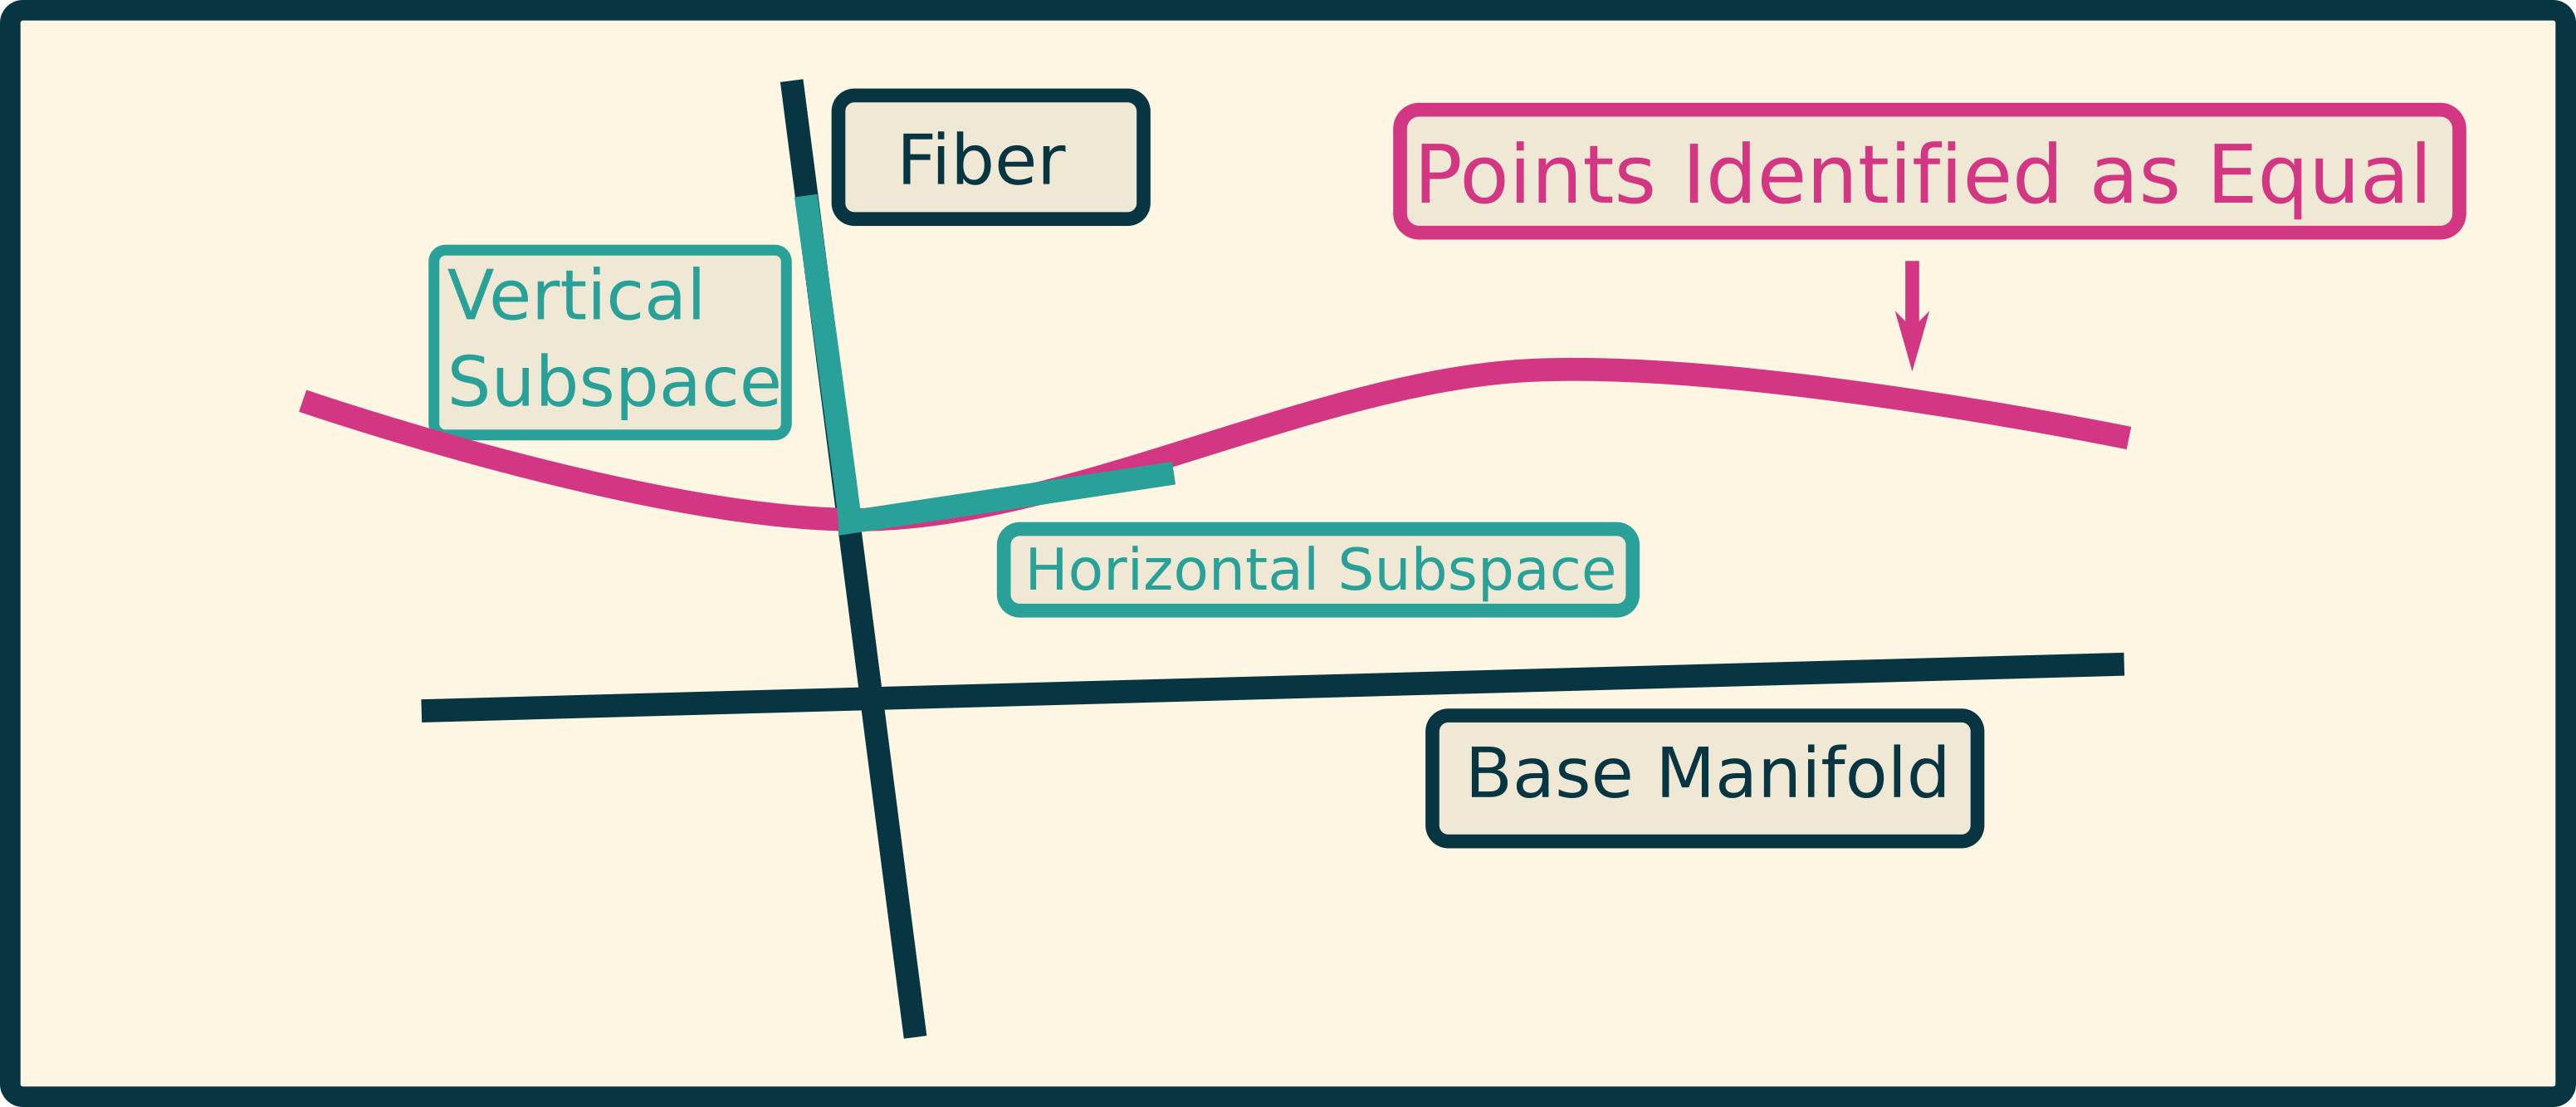
\includegraphics[width=\textwidth]{pics/bundle_tangent.png}
  \caption{Once we identify which points in the topology are identical, we can seperate out the tangent space at each point into the horizontal and vertical components.}
  \label{fig:bundle_tangent}
\end{figure}

Identifying 

%\chapter{Applying to Physics}
\section{Berry Connection}

The first person, Berry, to create a connection in condensed matter physics did so purely from a physics standpoint.  Only from discussions with Berry did Barry Simon make the jump from the physics formulas to the mathematical notions of parallel transport on a fiber bundle.

Here I replicate Berry's derivation.

Let's start with Schr\"odinger's equation, where the Hamiltonian depends on a set of parameters $\mathbf{R}(t)$ that we can manipulate in time.
\begin{equation}
  H(\mathbf{R}(t))\ket{\Psi(t)} = i \hbar \d{}{t}\ket{\Psi(t)}
\end{equation}

Next, we use the adiabatic theorem and assume that the parameters $\mathbf{R}(t)$ change slowly enough that we are always in an instantaneous eigenstate.  This holds as long as the frequency with which the Hamiltonian changes is much less than the energy between eigenstates.

Once we apply this approximation, we can break the rate of change for an eigenstate into the standard phase evolution and a slower evolution due to the evolution of the parameters.  All the while, this still is an eigenstate.
\begin{equation}
  E_n(\mathbf{R}(t)) \ket{n(\mathbf{R}(t))}
  =
  \hbar \left( \d{}{t} \theta(t) \right) \ket{n(\mathbf{R}(t))}
  +i \hbar \d{}{t}\ket{n(\mathbf{R}(t))}
\end{equation}
We multiply by corresponding bra to get this formula in a more convenient form,
\begin{equation}
  E_n(\mathbf{R}(t))=
  \hbar \left( \d{}{t}\theta(t) \right)
  + i \hbar \bra{n(\mathbf{R}(t))} \d{}{t} \ket{n(\mathbf{R}(t))}
\end{equation}
And now integrate the phase over time.
\begin{equation}
  \theta(t)=
  \frac{1}{\hbar}\int_{0}^{t}E_n(\mathbf{R}(t^{\prime}))dt^{\prime}
  -
  i \int_{0}^{t} \bra{n(\mathbf{R}(t^{\prime}))} \d{}{t^{\prime}} \ket{n(\mathbf{R}(t^{\prime}))} dt^{\prime}
\end{equation}
The first integral is the same time evolution phase we see all the time, but the second term, we can do something with that. Let's rewrite,
\begin{equation}
  \gamma
  =i \int_{0}^{t_{end}} \bra{n(\mathbf{R}(t^{\prime}))} \grad_{\mathbf{R}} \ket{n(\mathbf{R}(t^{\prime}))} \cdot \d{\mathbf{R}}{t^{\prime}} dt^{\prime}
  =i \int_{C} \bra{n(\mathbf{R})} \grad_{\mathbf{R}} \ket{n(\mathbf{R})} \cdot d \mathbf{R}
\end{equation}
From that equation we can extract
\begin{equation}
  A^{R^i} = \bra{n(\mathbf{R})} \grad_{\mathbf{R}} \ket{n(\mathbf{R})}
  \qquad \qquad \gamma= i \int_C A^{R^i} \cdot dR^i
\end{equation}


\begin{appendices}
\chapter{Notation}\label{ch:notation}
I understand not everyone will have the same amount of mathematical training, and though I do use pictures and handwaving, I don't shy away from formal definitions and notation.  Precision is necessary.  So here, I will cover some of the symbols and phrases that I usually take from granted people know.

\begin{definition}[Exists]
  $\exists$ is shorthand for "there exists".  It does not make any constraints on the object other than existance.
\end{definition}

\begin{definition}[For all]
  $\forall$ is shorthand for "for all".  Often used in definitions or constraints.
\end{definition}

\begin{definition}[In]
  For members of a set, I will use $\in$ to denote membership.  For example, apples $\in$ fruits.
\end{definition}

\begin{definition}[Implies]
  I will use $\rightarrow$ is we can logically deduce one thing from another.
\end{definition}

\subsection{Notation for Special Sets}
\begin{enumerate}
  \item $\mathbb{R}$ the Real line, for example, 1, $\pi$, $\sqrt{2}$, $569543/3874329$, and $.3234898957786...$
  \item $\mathbb{Z}$ the Integers: $-1, 0, 1, 2,...$
  \item $\mathbb{Q}$ The Rationals: any number that can be written as the ratio of two integers $p/q : p,q \in \mathbb{Z}$.
  \item $S^1$ The points on on the surface of a circle.
  \item $S^2$ The points on the surface of a sphere.
  \item $S^n$ The points on the surface on an n-sphere.  I hope you get the trend now.
\end{enumerate}

\end{appendices}
%\bibliography{biblio}
%\bibliographystyle{unsrt}
\end{document}
